

\begin{figure*}[h]
    \centering
    \begin{subfigure}[b]{0.95\textwidth} 
        \centering
        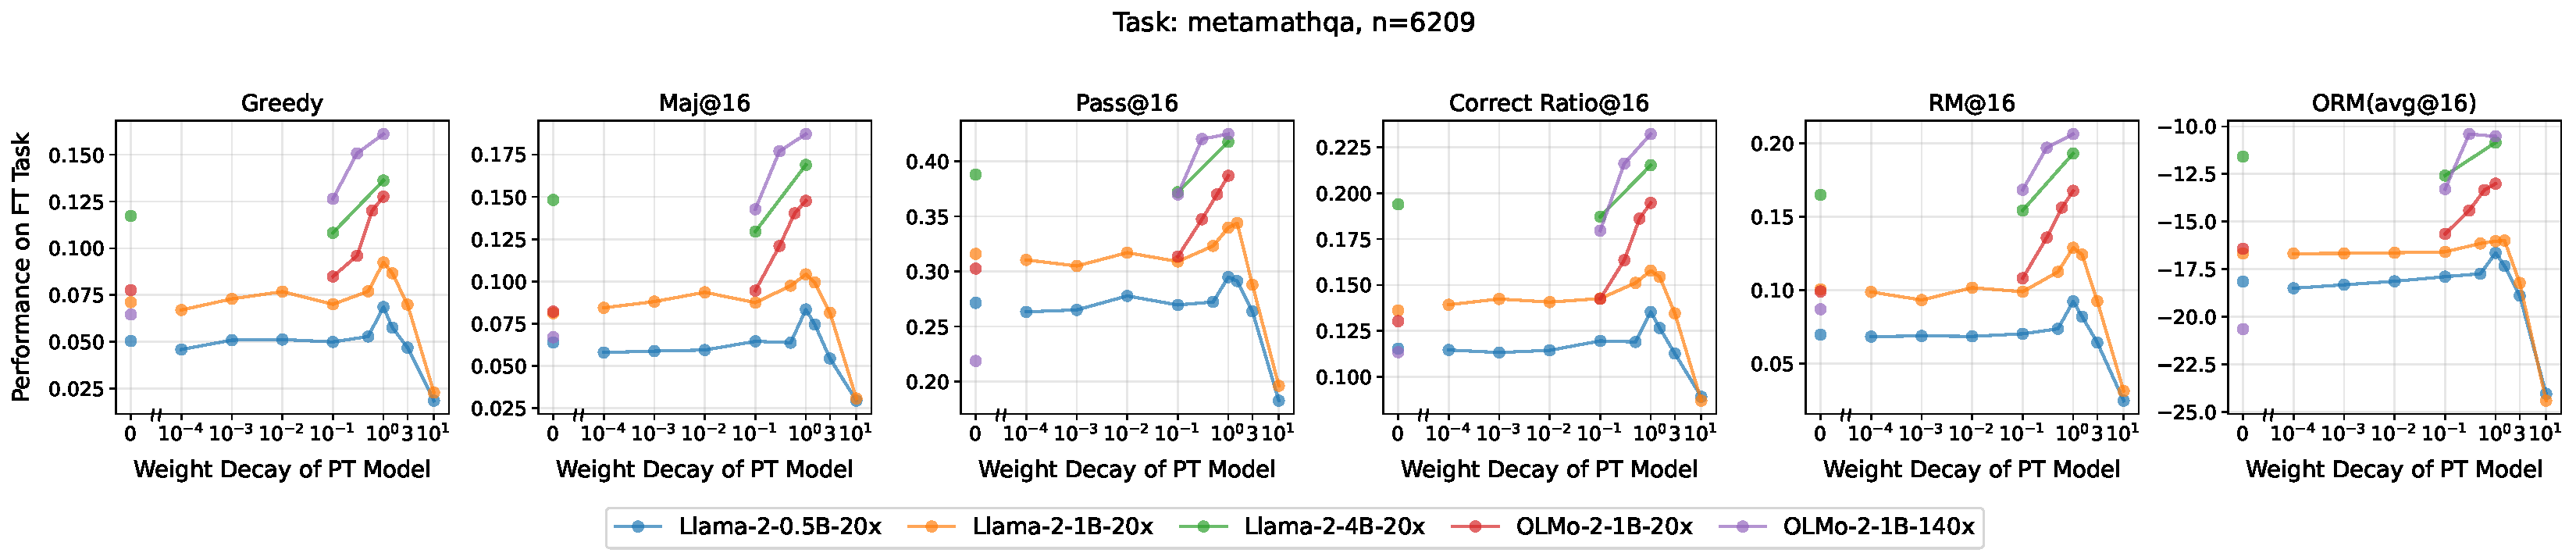
\includegraphics[width=\linewidth, trim={0 17mm 0 20mm}, clip]{figs/a01_ft_cot/aggregate_tasks/all_models_withwd0_metamathqa.pdf}
        \caption{\metamathqa{}}
    \end{subfigure}
    \begin{subfigure}[b]{0.95\textwidth} 
        \centering
        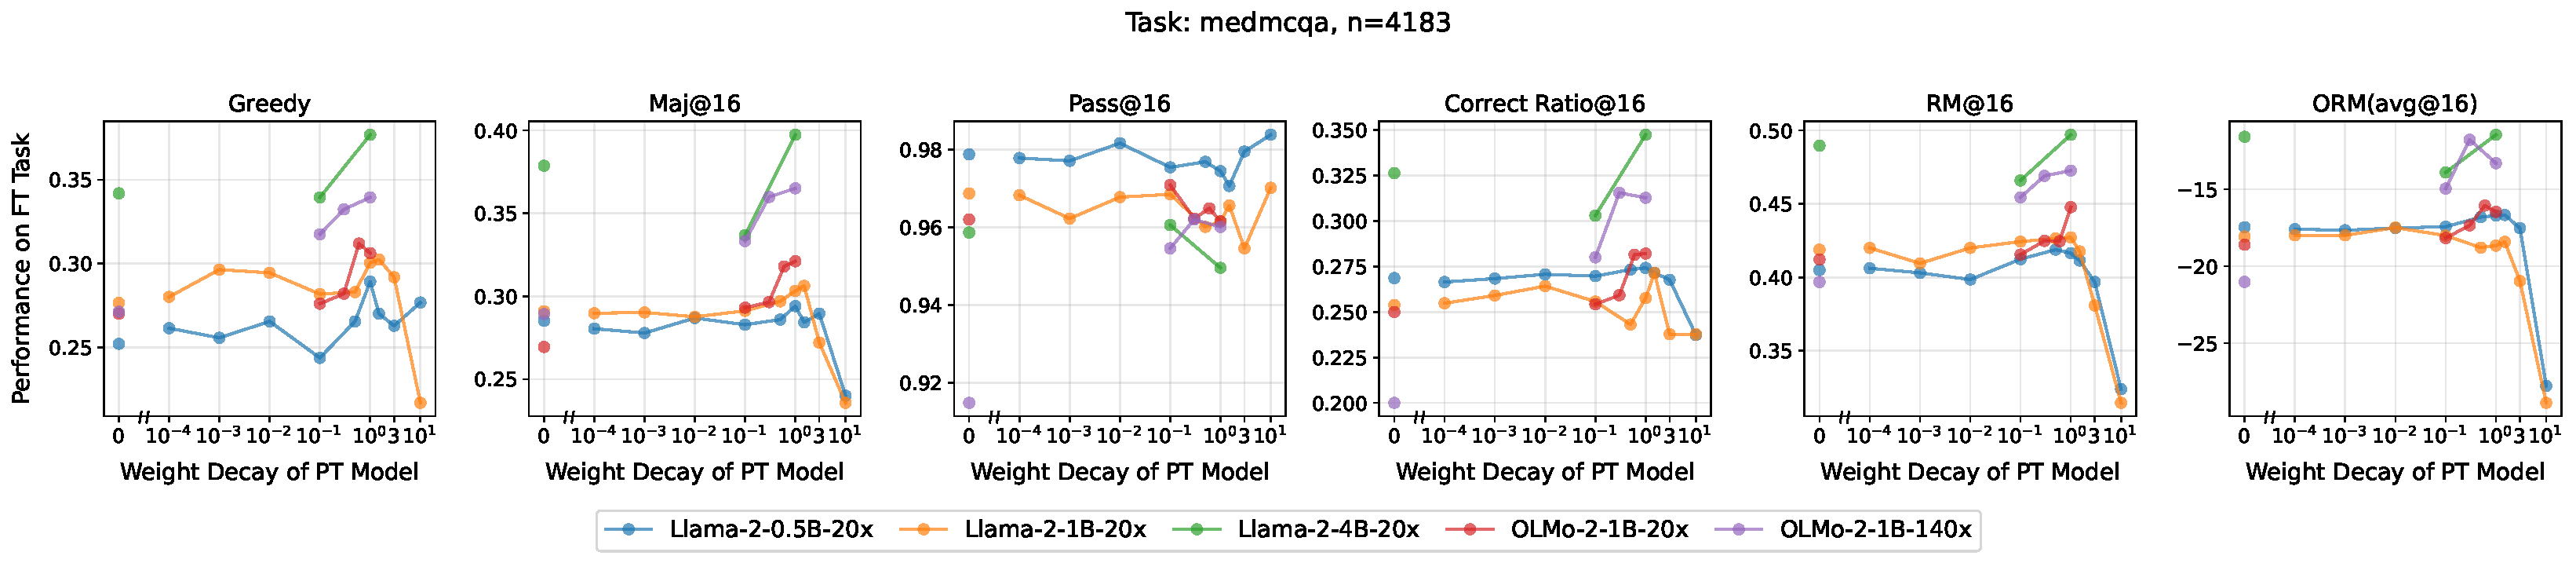
\includegraphics[width=\linewidth, trim={0 17mm 0 20mm}, clip]{figs/a01_ft_cot/aggregate_tasks/all_models_withwd0_medmcqa.pdf} 
        \caption{\medmcqa{}}
    \end{subfigure}
    \begin{subfigure}[b]{0.95\textwidth} 
        \centering
        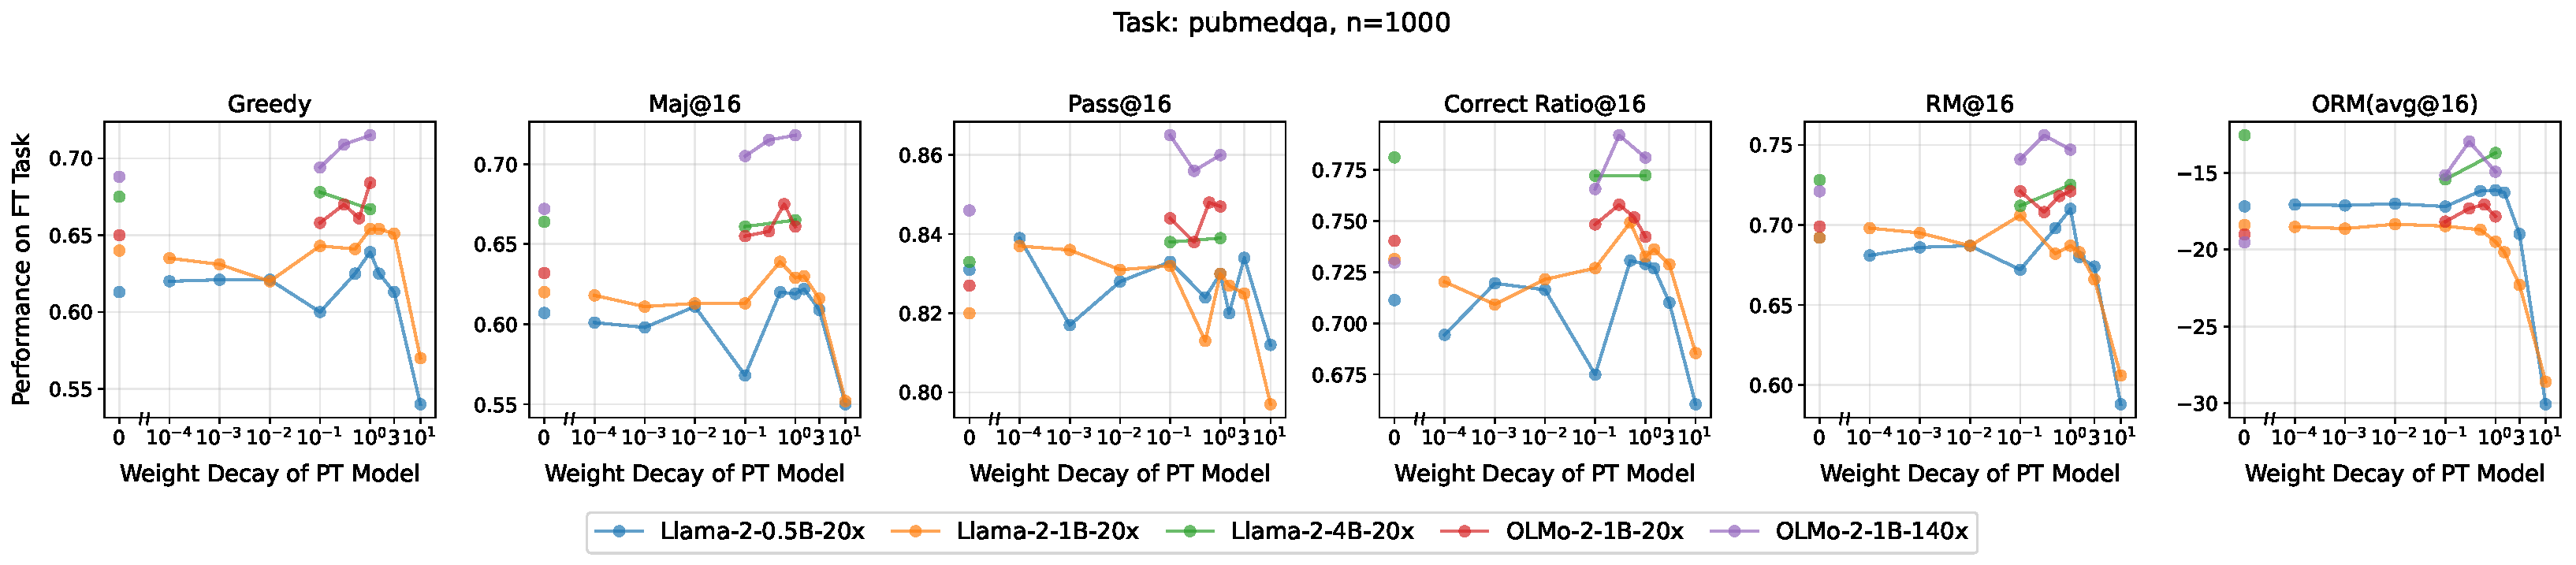
\includegraphics[width=\linewidth, trim={0 17mm 0 20mm}, clip]{figs/a01_ft_cot/aggregate_tasks/all_models_withwd0_pubmedqa.pdf} 
        \caption{\pubmedqa{}}
    \end{subfigure}
    \begin{subfigure}[b]{0.95\textwidth} 
        \centering
        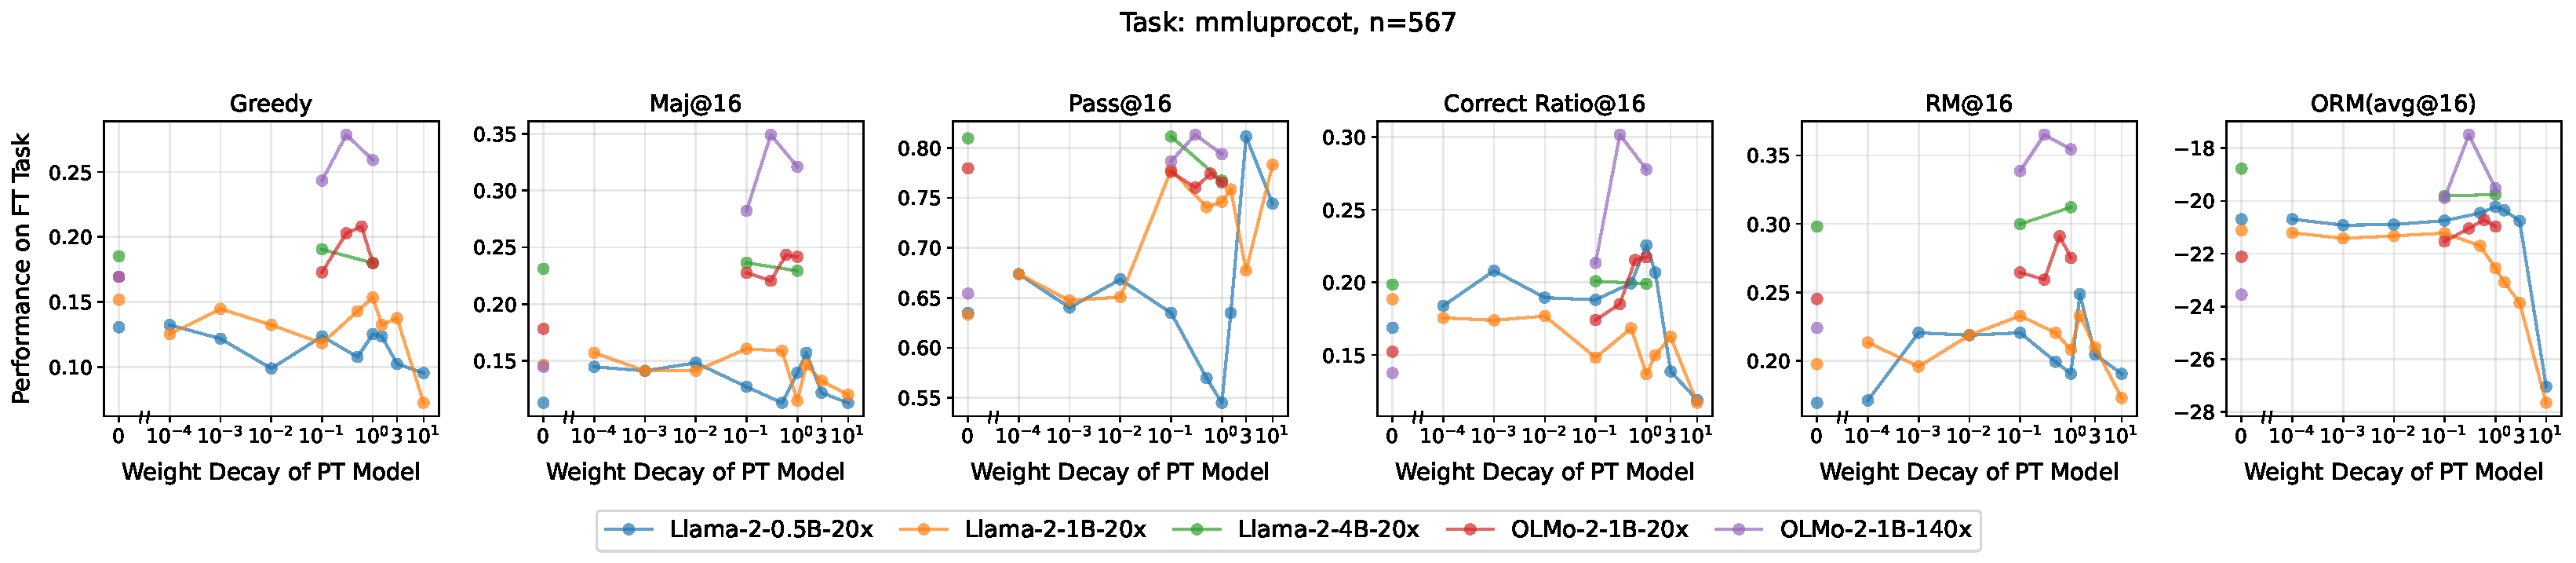
\includegraphics[width=\linewidth, trim={0 17mm 0 20mm}, clip]{figs/a01_ft_cot/aggregate_tasks/all_models_withwd0_mmluprocot.pdf} 
        \caption{\mmluprocot{}}
    \end{subfigure}
    \begin{subfigure}[b]{0.95\textwidth} 
        \centering
        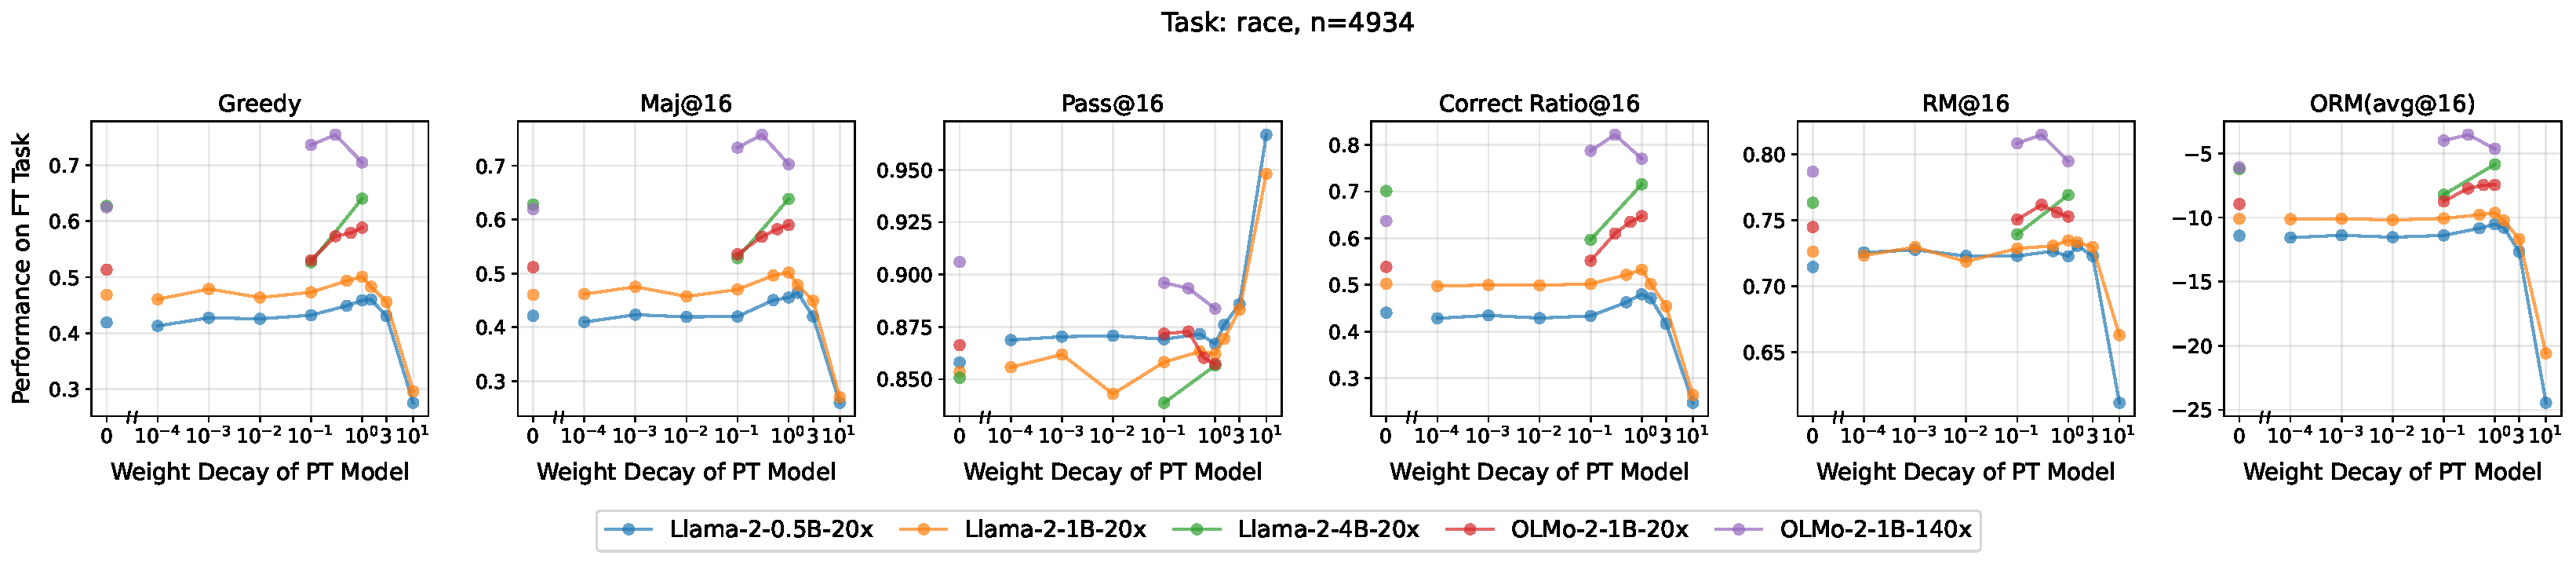
\includegraphics[width=\linewidth, trim={0 17mm 0 20mm}, clip]{figs/a01_ft_cot/aggregate_tasks/all_models_withwd0_race.pdf} 
        \caption{\race{}}
    \end{subfigure}
    \begin{subfigure}[b]{0.95\textwidth} 
        \centering
        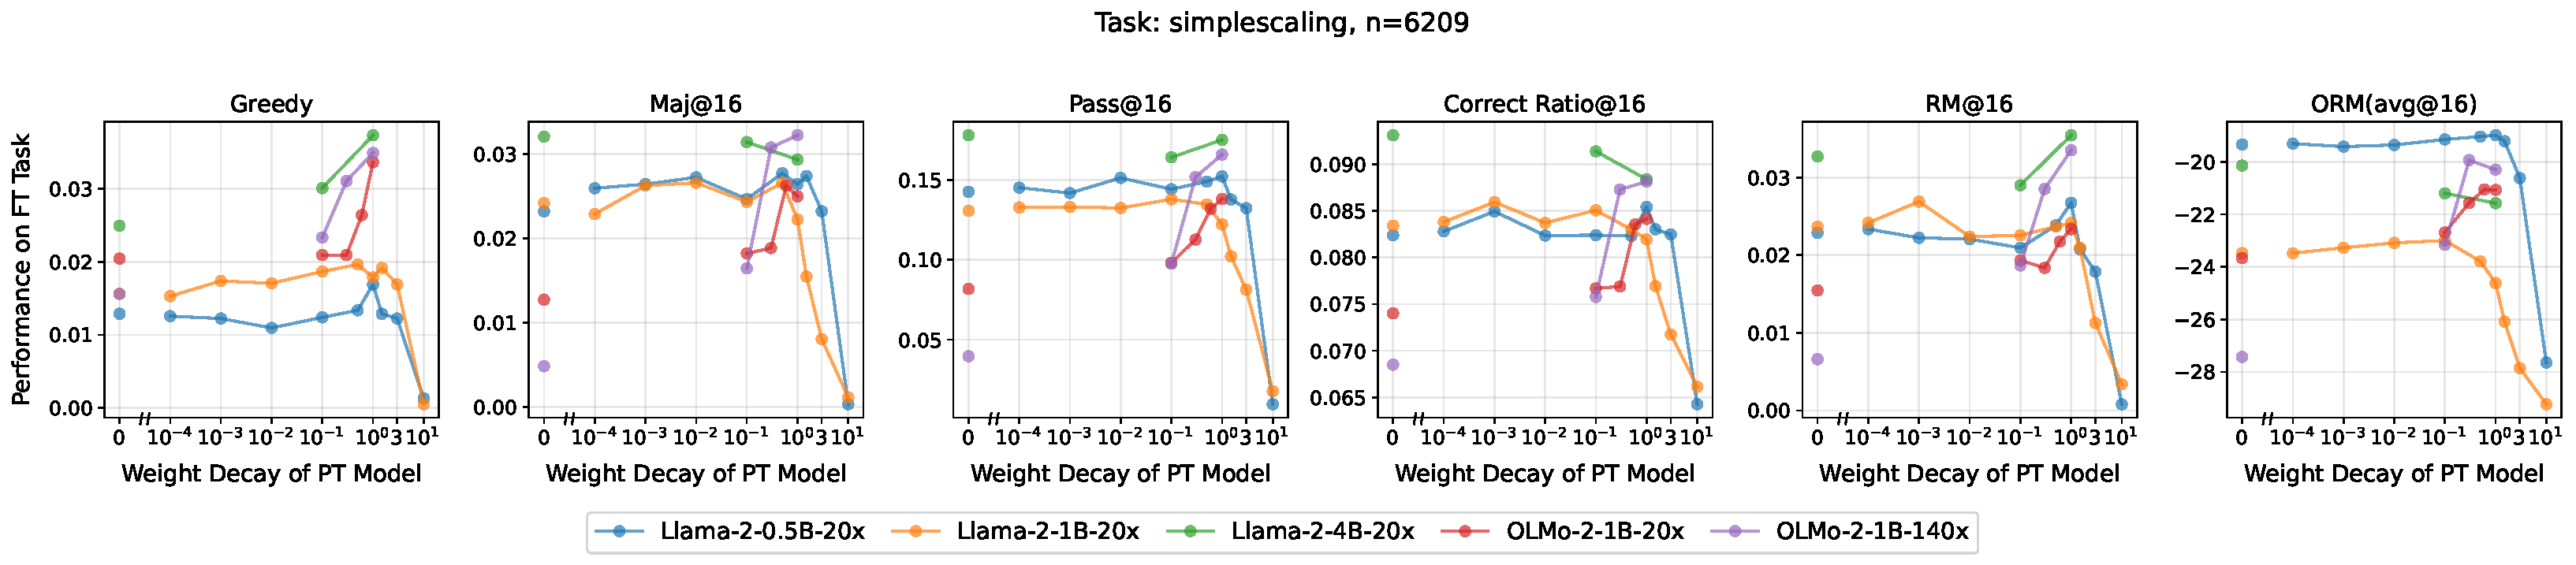
\includegraphics[width=\linewidth, trim={0 17mm 0 20mm}, clip]{figs/a01_ft_cot/aggregate_tasks/all_models_withwd0_simplescaling.pdf} 
        \caption{\simplescaling{}}
    \end{subfigure}
    \begin{subfigure}[b]{0.95\textwidth} 
        \centering
        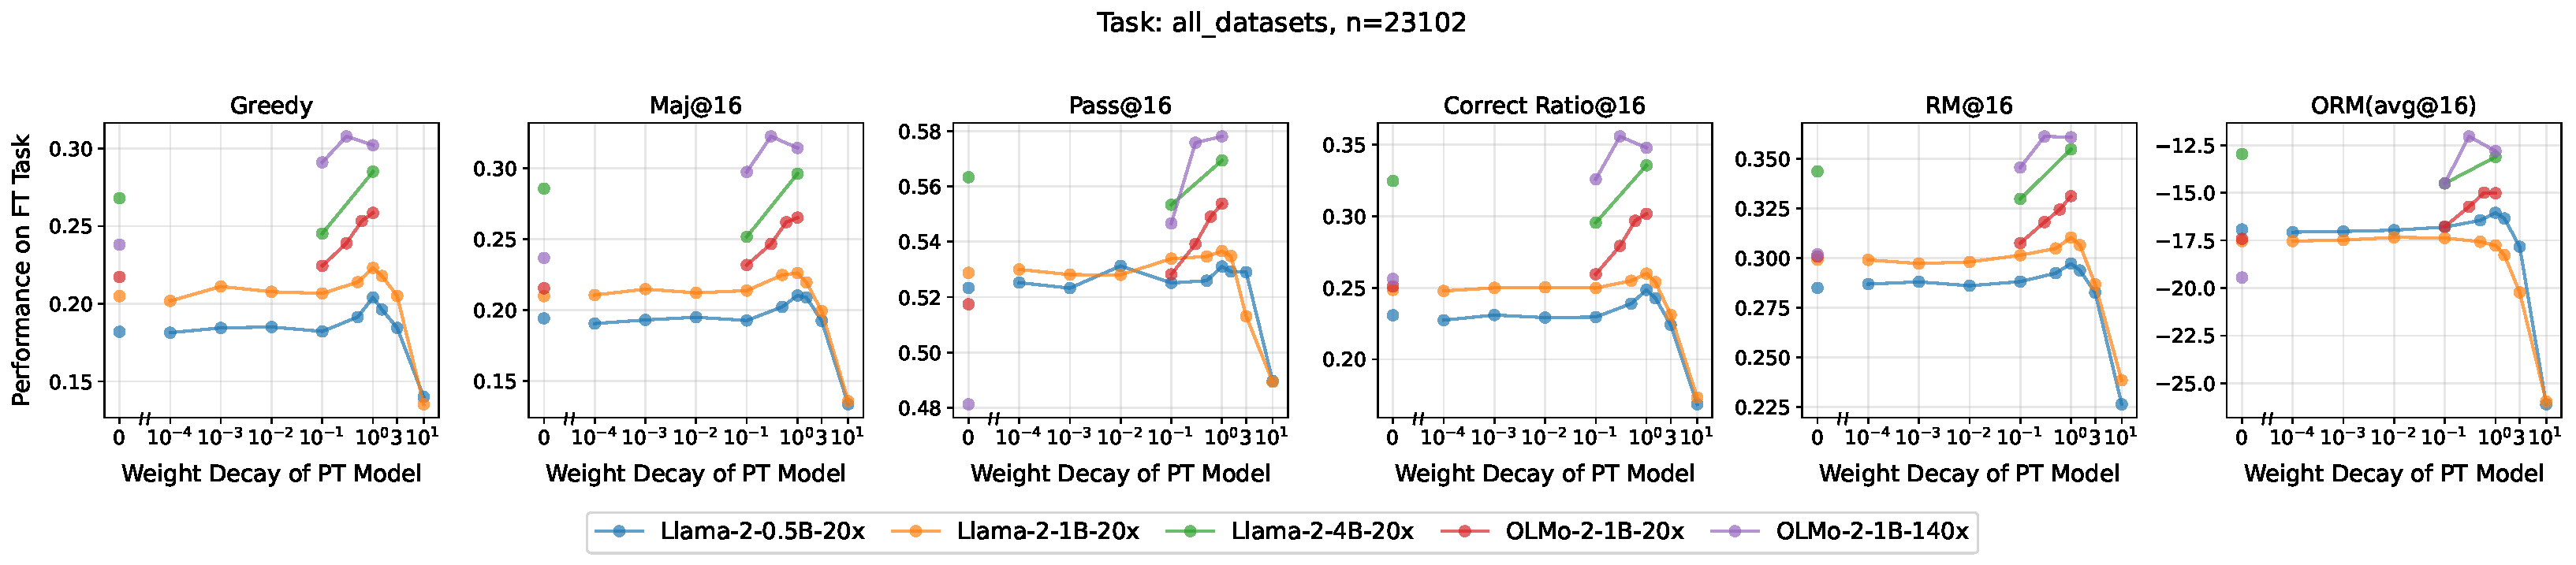
\includegraphics[width=\linewidth, trim={0 0 0 20mm}, clip]{figs/a01_ft_cot/aggregate_tasks/all_models_withwd0_all_datasets.pdf} 
        \caption{Average over datasets}
    \end{subfigure}
    \caption{{\bf Fine-tuning performance on chain-of-thought tasks.} Weight decay during pretraining improves model plasticity, leading to higher downstream performance.}
    \label{fig:app-wd-vs-ftperf-all-tasks}
\end{figure*}



\begin{figure*}[h] 
    \centering
    \begin{subfigure}[b]{0.88\textwidth} 
        \centering
        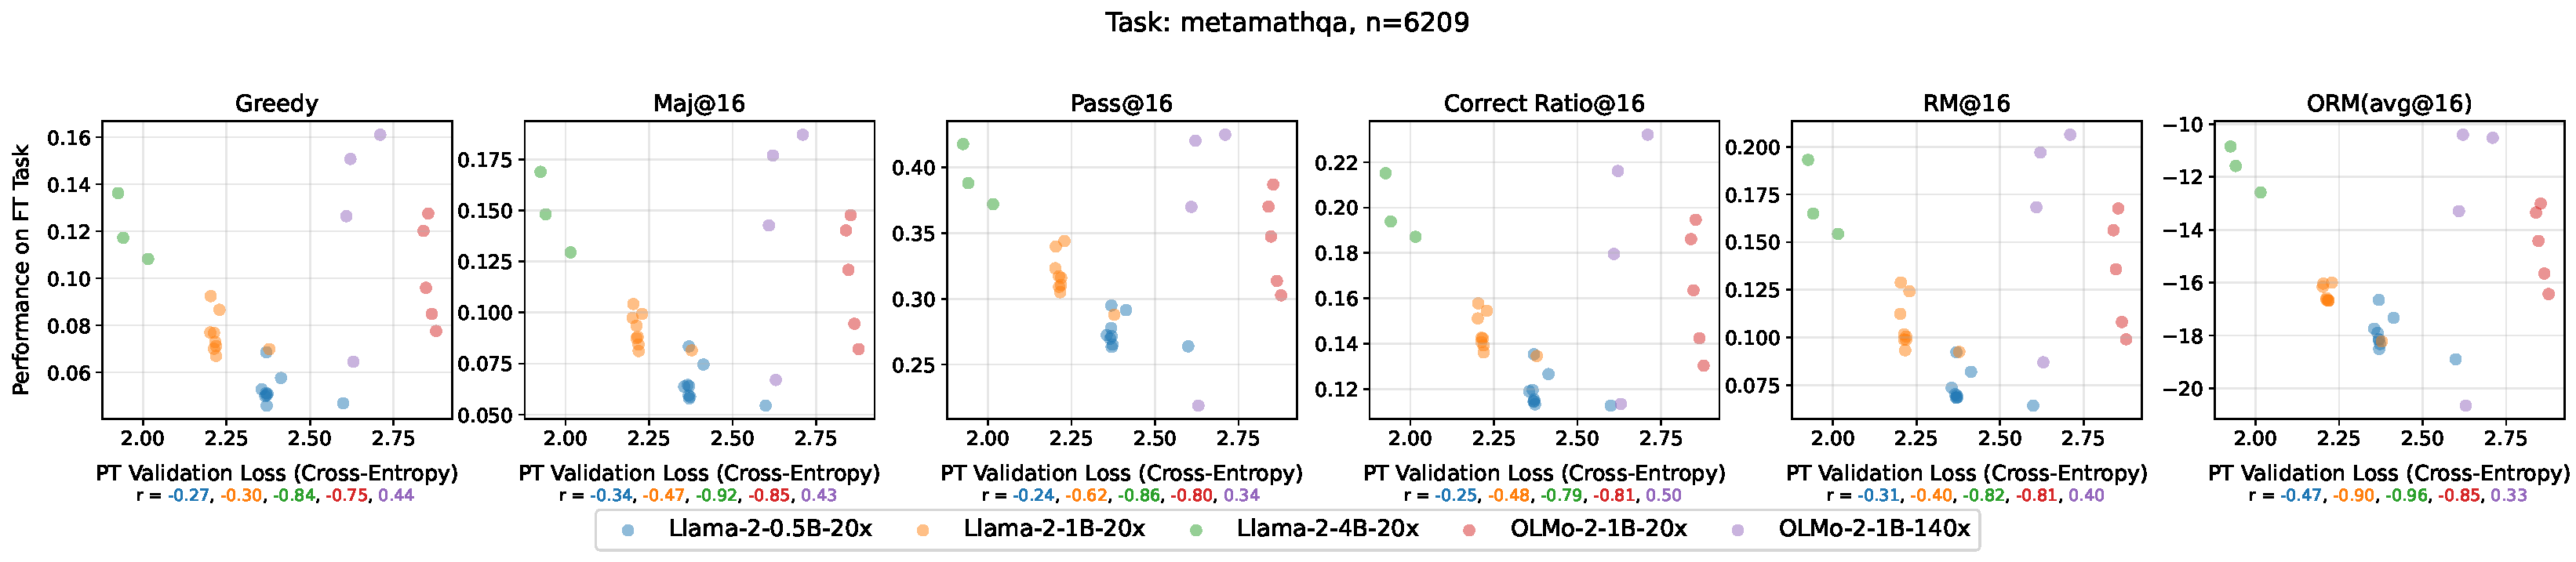
\includegraphics[width=\linewidth, trim={0 13mm 0 15mm}, clip]{figs/a04_val_loss/all_models_loss_vs_ft_acc_metamathqa.pdf}
    \caption{\metamathqa{}{}}
    \end{subfigure}
    \begin{subfigure}[b]{0.88\textwidth} 
        \centering
        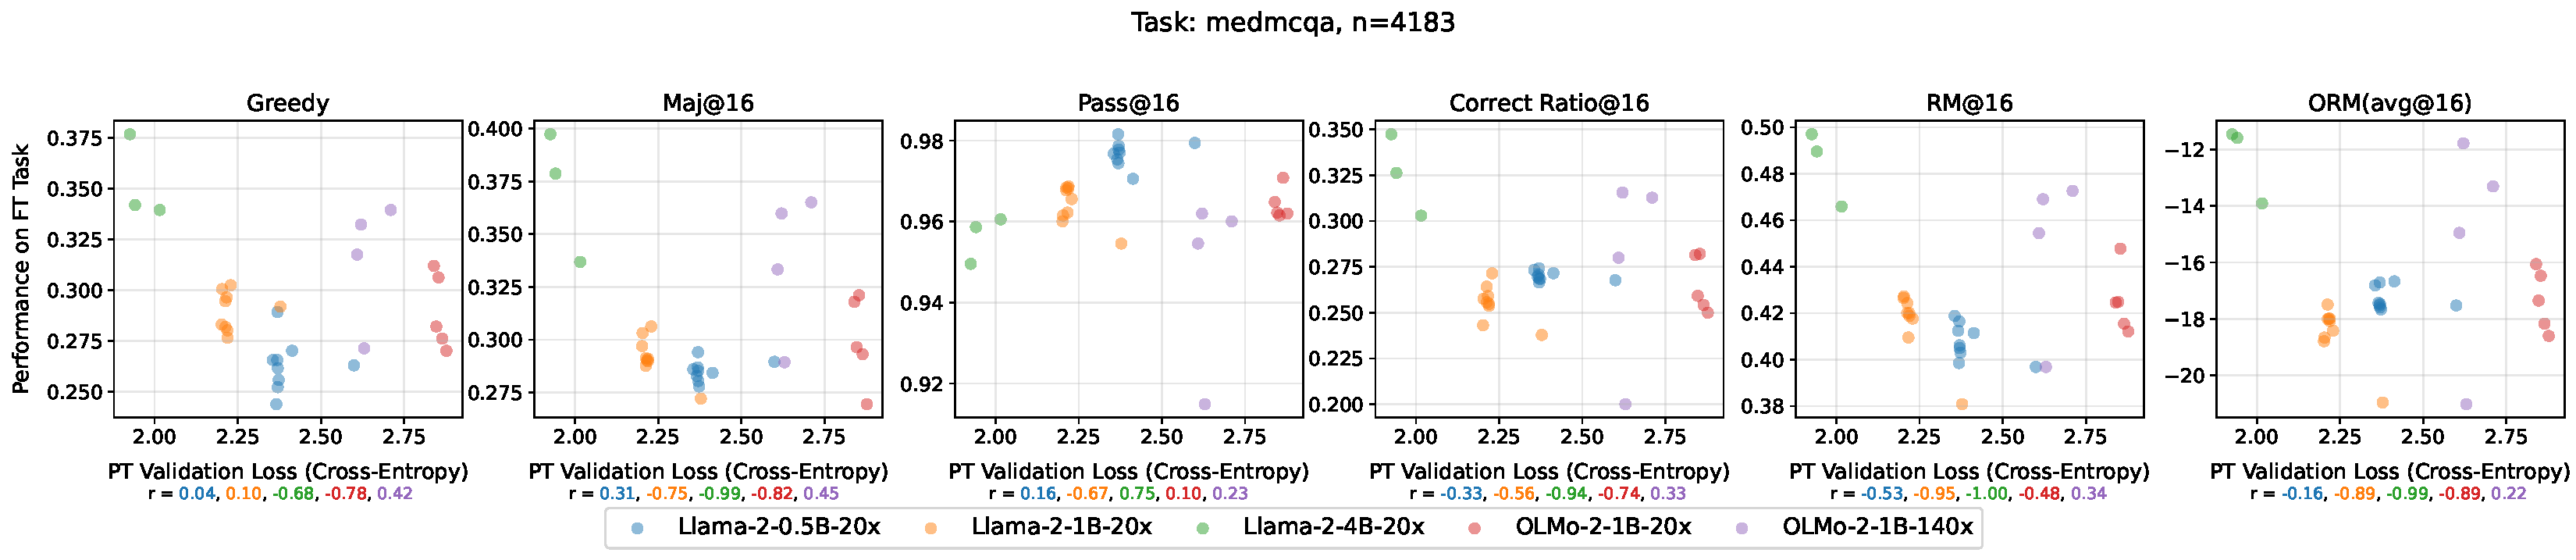
\includegraphics[width=\linewidth, trim={0 13mm 0 15mm}, clip]{figs/a04_val_loss/all_models_loss_vs_ft_acc_medmcqa.pdf}
    \caption{\medmcqa{}{}}
    \end{subfigure}
    \begin{subfigure}[b]{0.88\textwidth} 
        \centering
        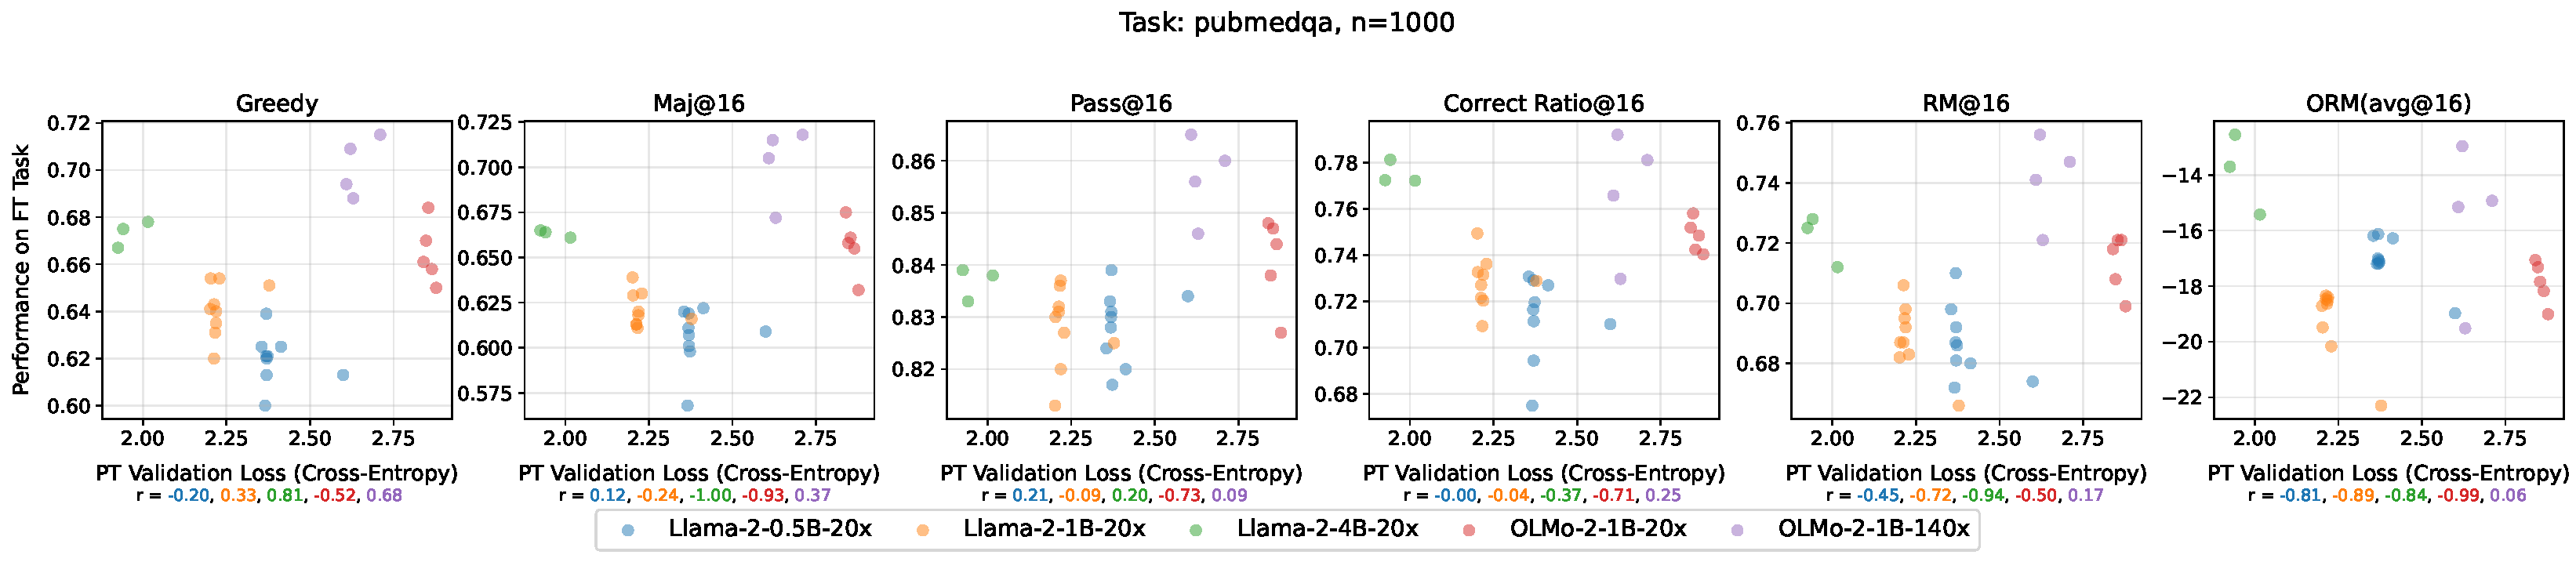
\includegraphics[width=\linewidth, trim={0 13mm 0 15mm}, clip]{figs/a04_val_loss/all_models_loss_vs_ft_acc_pubmedqa.pdf}
    \caption{\pubmedqa{}{}}
    \end{subfigure}
    \begin{subfigure}[b]{0.88\textwidth} 
        \centering
        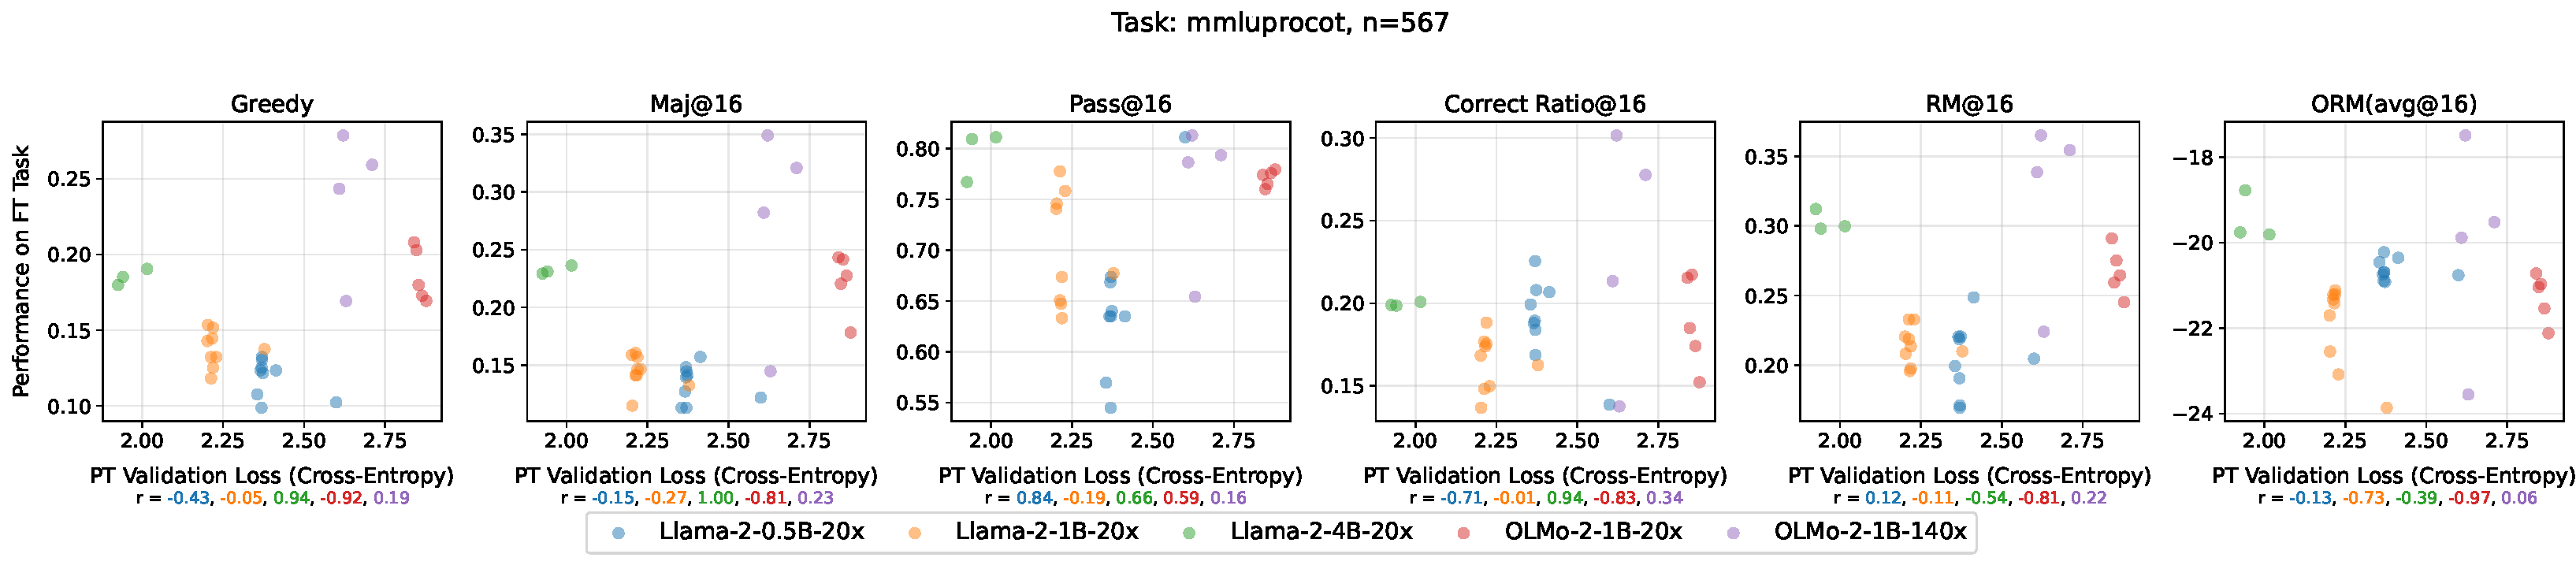
\includegraphics[width=\linewidth, trim={0 13mm 0 15mm}, clip]{figs/a04_val_loss/all_models_loss_vs_ft_acc_mmluprocot.pdf}
    \caption{\mmluprocot{}{}}
    \end{subfigure}
    \begin{subfigure}[b]{0.88\textwidth} 
        \centering
        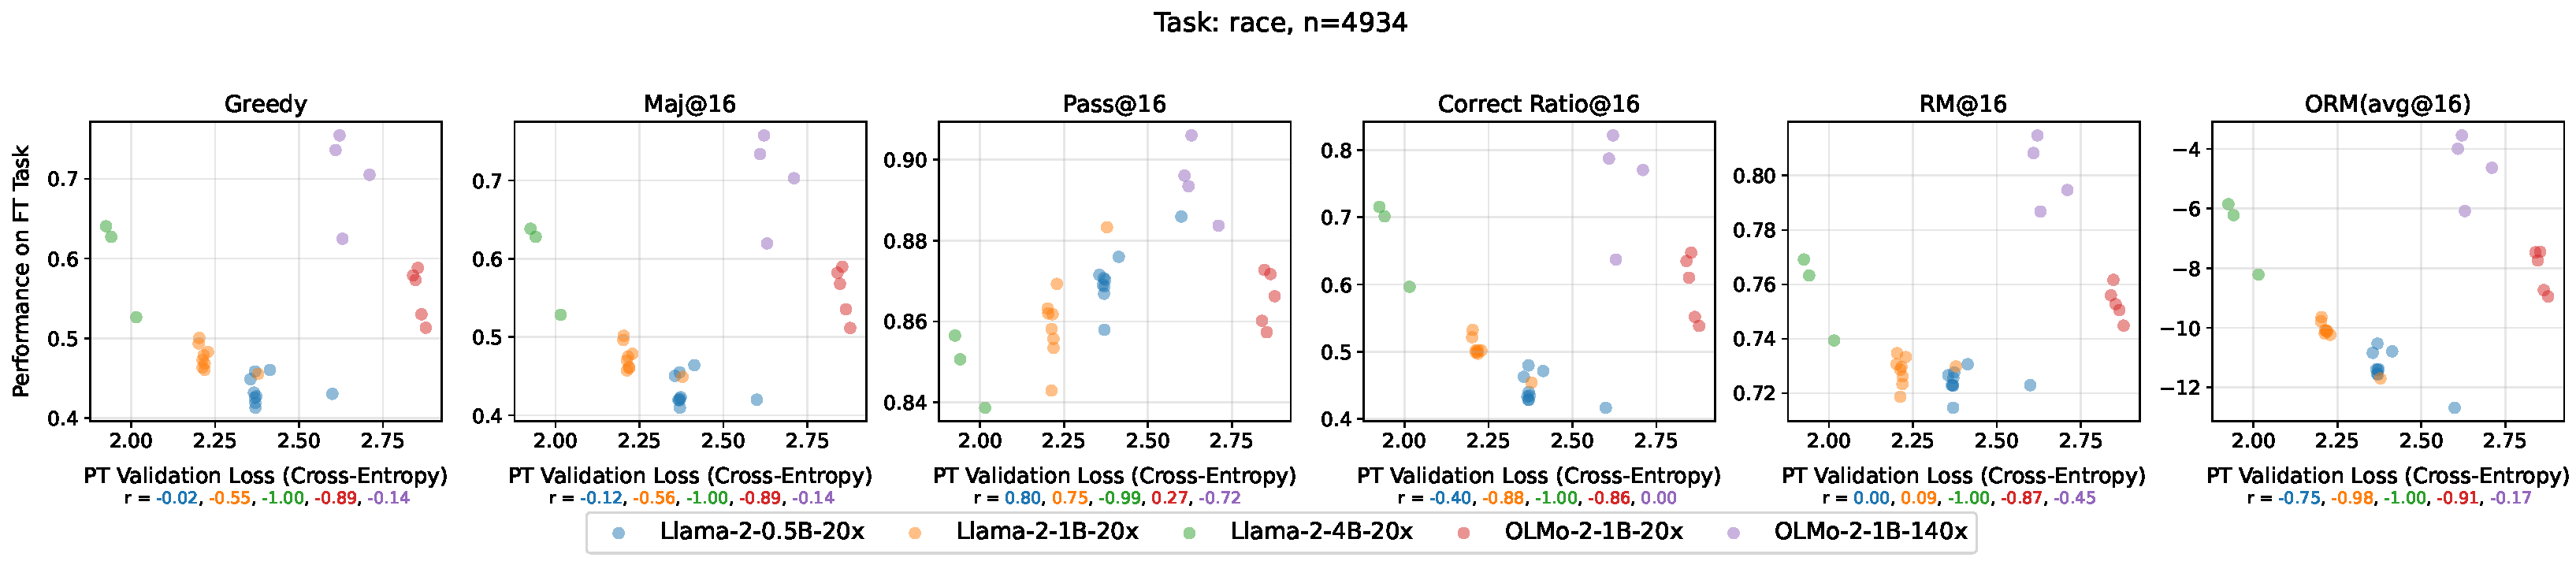
\includegraphics[width=\linewidth, trim={0 13mm 0 15mm}, clip]{figs/a04_val_loss/all_models_loss_vs_ft_acc_race.pdf}
    \caption{\race{}}
    \end{subfigure}
    \begin{subfigure}[b]{0.88\textwidth} 
        \centering
        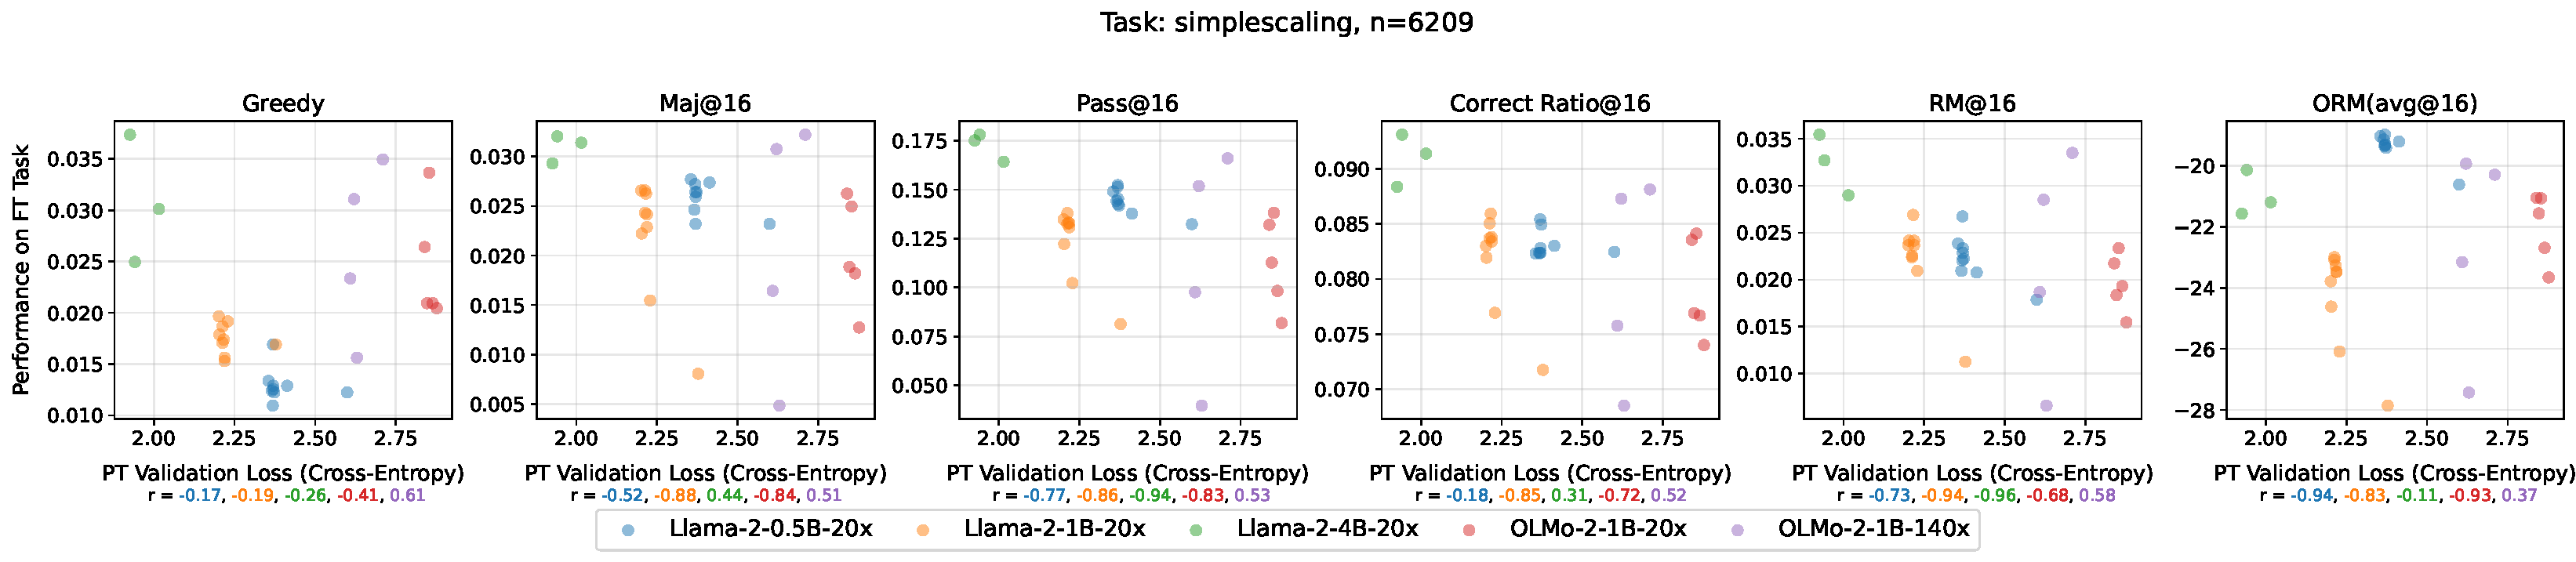
\includegraphics[width=\linewidth, trim={0 13mm 0 15mm}, clip]{figs/a04_val_loss/all_models_loss_vs_ft_acc_simplescaling.pdf}
    \caption{\simplescaling{}}
    \end{subfigure}
    \begin{subfigure}[b]{0.88\textwidth} 
        \centering
        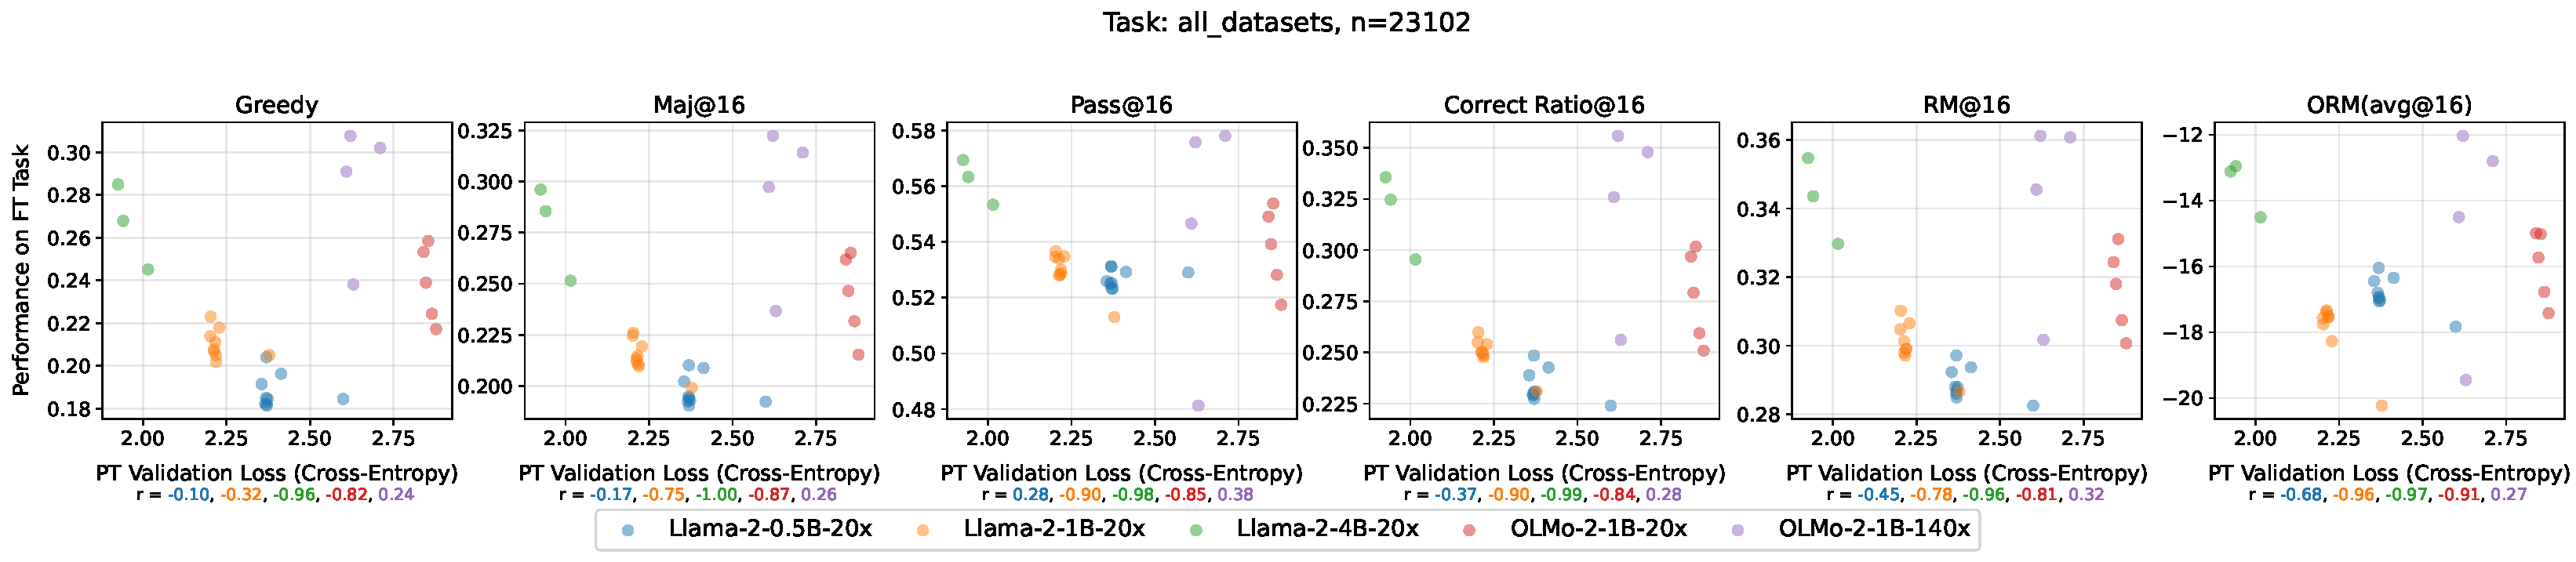
\includegraphics[width=\linewidth, trim={0 0 0 15mm}, clip]{figs/a04_val_loss/all_models_loss_vs_ft_acc_all_datasets.pdf}
    \caption{Average over datasets}
    \end{subfigure}
    \caption{{\bf Pretraining validation cross-entropy loss vs. fine-tuning accuracy for chain-of-thought tasks.} Pretraining validation cross-entropy loss (pretraining performance) is not fully predictive of model performance after fine-tuning (downstream performance).}
    \label{fig:app-ptloss-vs-ftperf-full}
\end{figure*}


\clearpage


\begin{figure}[h] 
    \centering
    \begin{subfigure}[b]{\textwidth} 
        \centering
        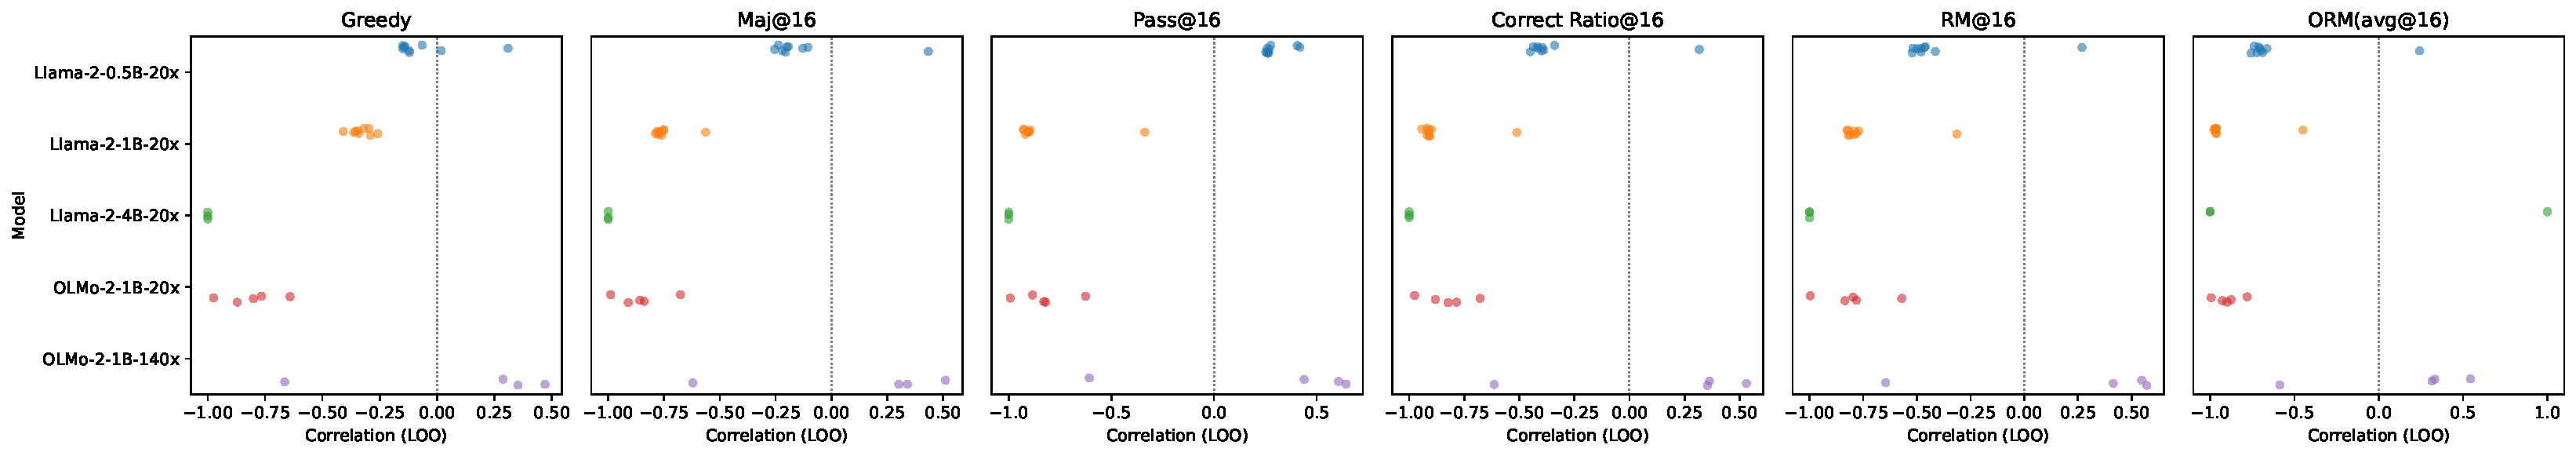
\includegraphics[width=\linewidth]{figs/a04_val_loss/r_loo.pdf}
    \end{subfigure}
    \caption{{\bf Stability analysis for Pearson correlation coefficient.} Pearson correlation is computed for each leave-one-out (LOO) subset in Figure~\ref{fig:app-ptloss-vs-ftperf-full}g. The LOO correlation can change noticeably in magnitude and sign, suggesting that the correlation for the full set of data points in Figure~\ref{fig:app-ptloss-vs-ftperf-full}g is rather unstable, which further supports the finding in that pretraining validation cross-entropy loss (pretraining performance) is not perfectly predictive of fine-tuning accuracy (downstream performance).} 
    \label{fig:app-r-loo}
\end{figure}



\begin{figure*}[h]
    \centering
    % Row 1
    \begin{subfigure}[b]{0.29\textwidth}
        \centering
        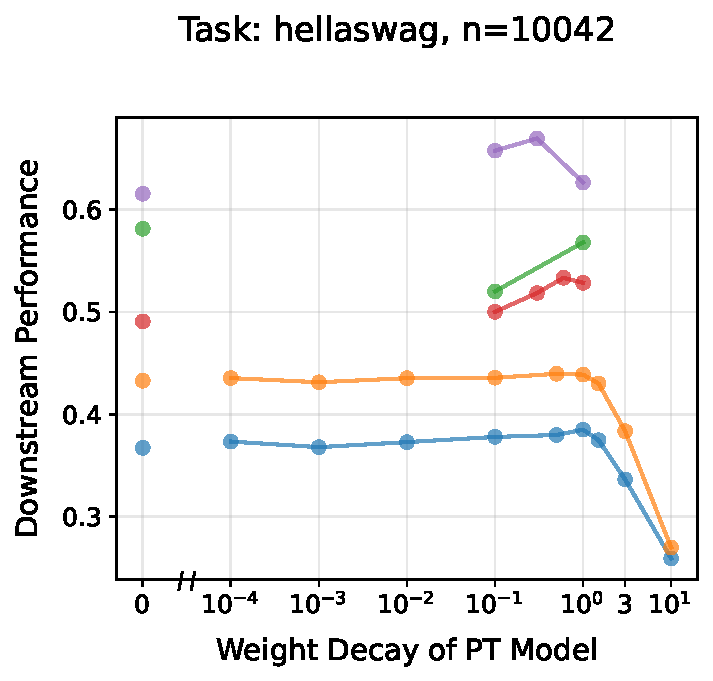
\includegraphics[
            width=\linewidth,
            trim={0 0 0 30},
            clip
            ]{figs/a09_ft_lang/withwd0_hellaswag.pdf}
        \caption{\hellaswag{}}
    \end{subfigure}
    \hfill
    \begin{subfigure}[b]{0.29\textwidth}
        \centering
        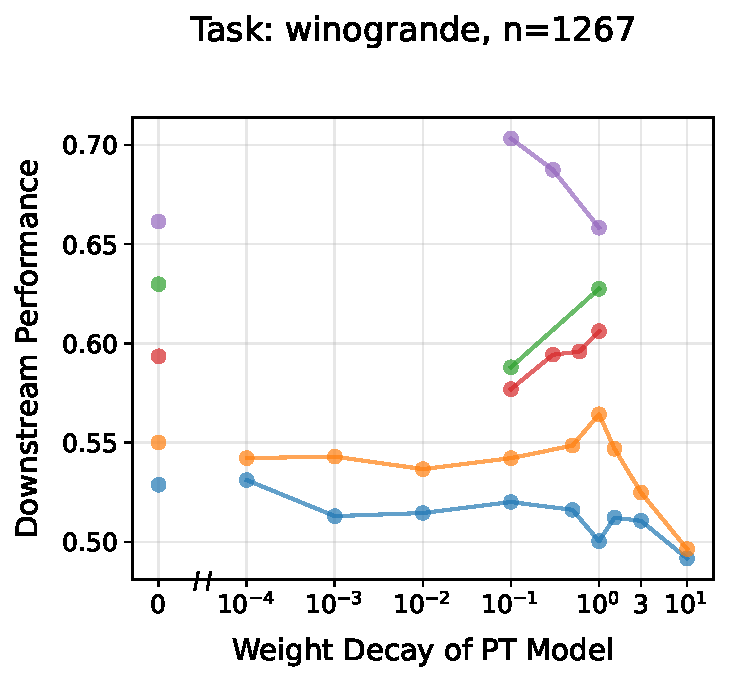
\includegraphics[
            width=\linewidth,
            trim={0 0 0 30},
            clip
            ]{figs/a09_ft_lang/withwd0_winogrande.pdf}
        \caption{\winogrande{}}
    \end{subfigure}
    \hfill
    \begin{subfigure}[b]{0.29\textwidth}
        \centering
        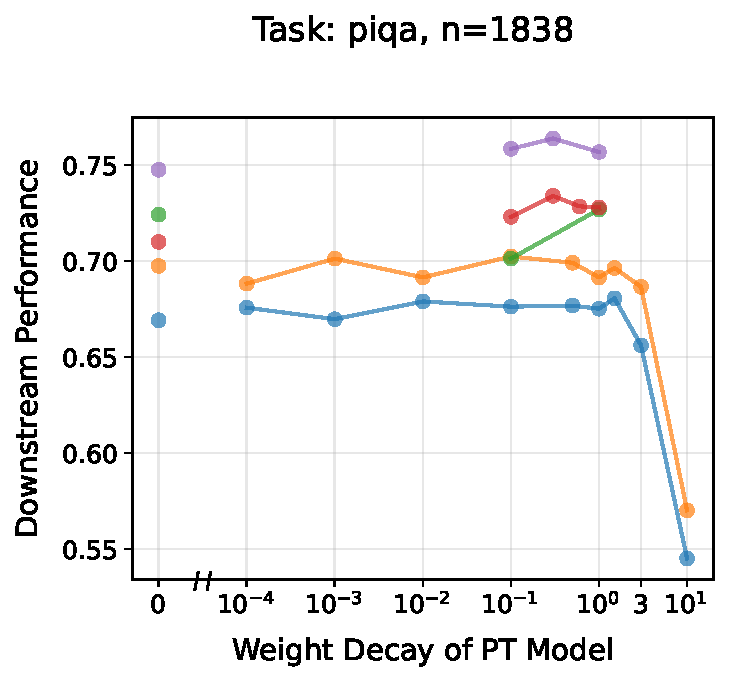
\includegraphics[
            width=\linewidth,
            trim={0 0 0 30},
            clip
            ]{figs/a09_ft_lang/withwd0_piqa.pdf}
        \caption{\piqa{}}
    \end{subfigure}
    \vspace{6pt}
    % Row 2
    \begin{subfigure}[b]{0.29\textwidth}
        \centering
        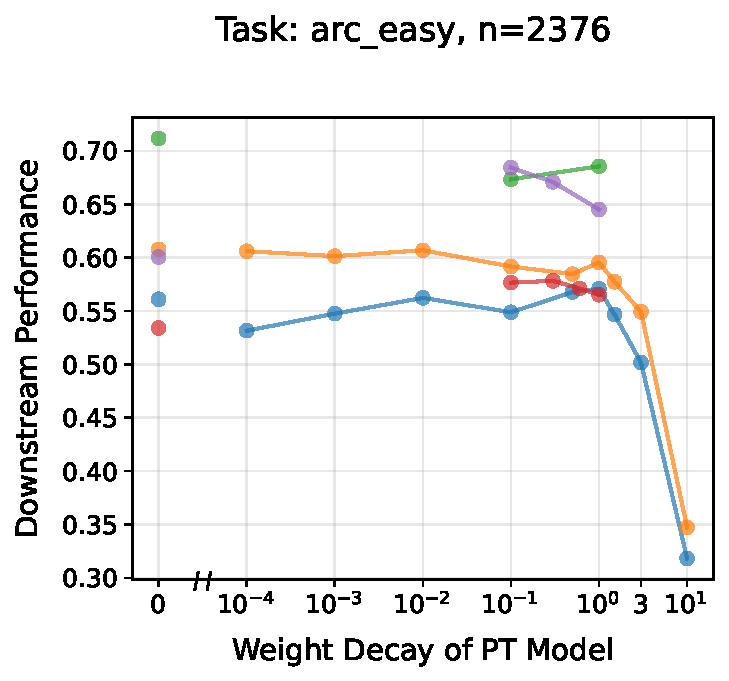
\includegraphics[
            width=\linewidth,
            trim={0 0 0 30},
            clip
            ]{figs/a09_ft_lang/withwd0_arc_easy.pdf}
        \caption{\arceasy{}}
    \end{subfigure}
    \hfill
    \begin{subfigure}[b]{0.29\textwidth}
        \centering
        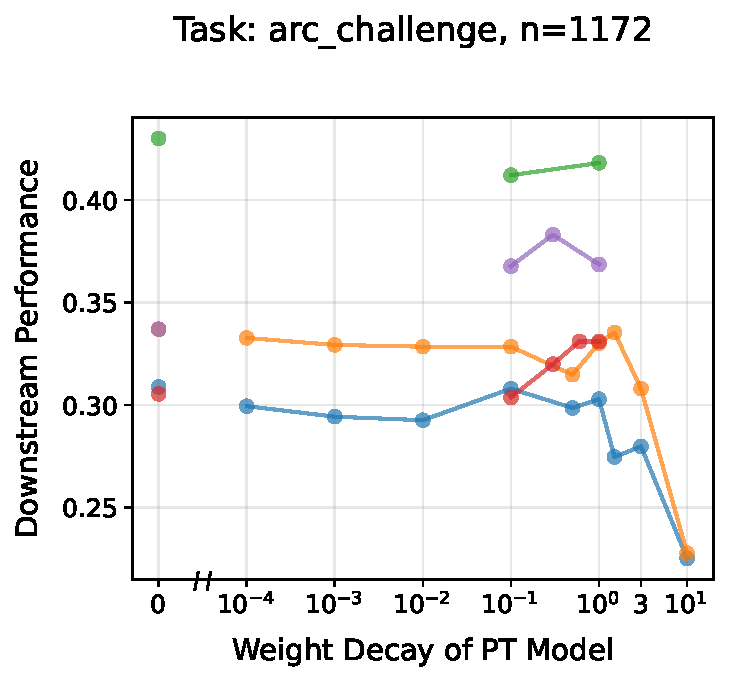
\includegraphics[
            width=\linewidth,
            trim={0 0 0 30},
            clip
            ]{figs/a09_ft_lang/withwd0_arc_challenge.pdf}
        \caption{\arcchallenge{}}
    \end{subfigure}
    \hfill
    \begin{subfigure}[b]{0.29\textwidth}
        \centering
        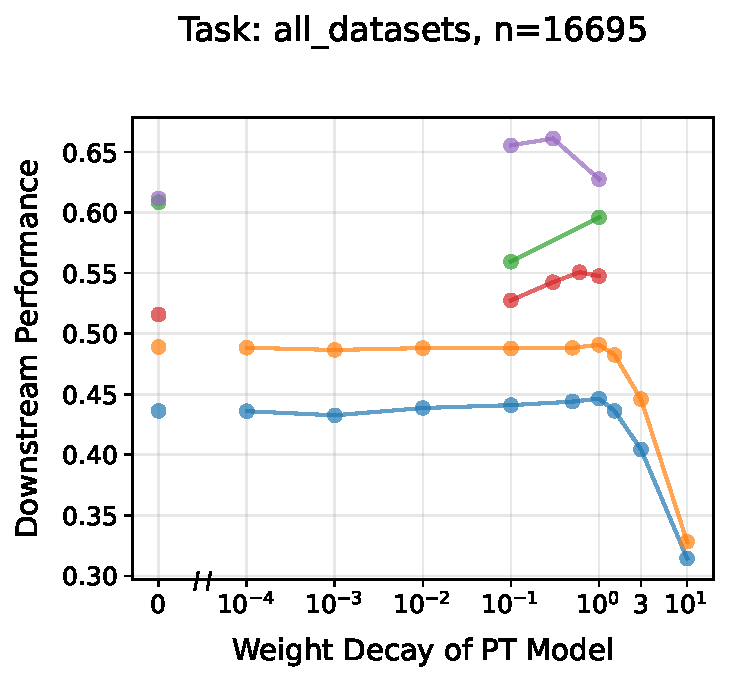
\includegraphics[
            width=\linewidth,
            trim={0 0 0 30},
            clip
            ]{figs/a09_ft_lang/withwd0_all_datasets.pdf}
        \caption{Average over datasets}
    \end{subfigure}
    
\includegraphics[width=0.8\linewidth]{figs/a04_val_loss/legend.pdf}
    \caption{{\bf Fine-tuning performance on language and general knowledge tasks.} Weight decay during pretraining improves model plasticity, leading to higher downstream performance.}
    \label{fig:app-ft-lang}
\end{figure*}




\vspace{0.4cm}
\begin{center}
    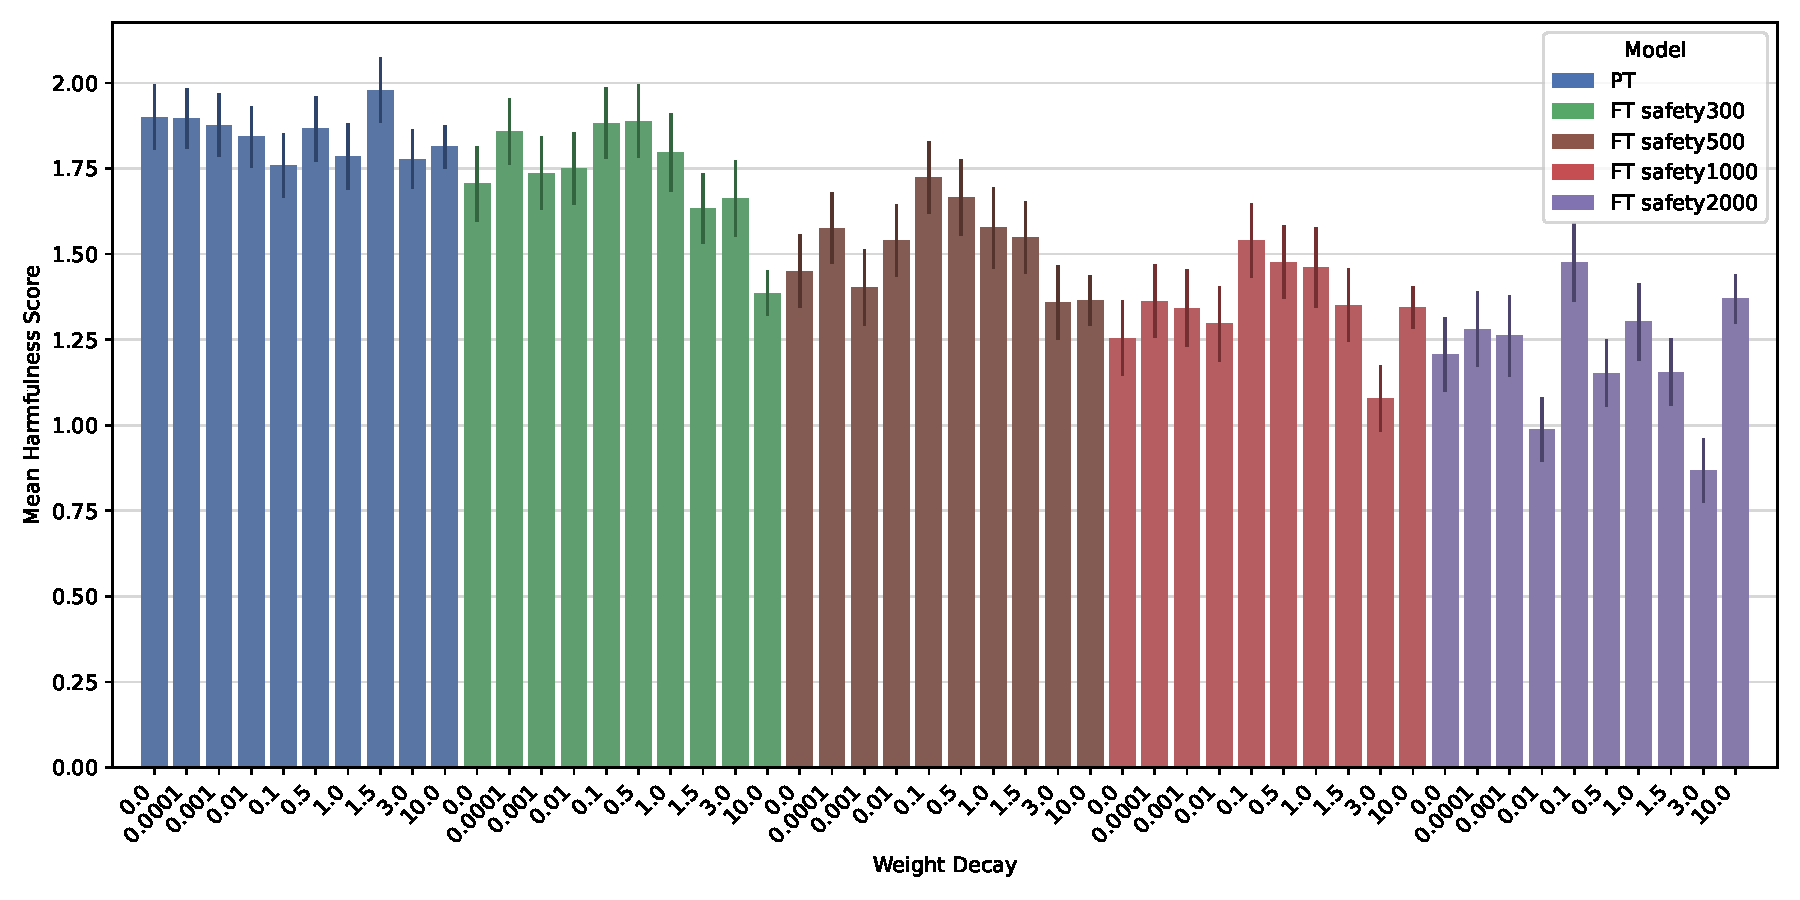
\includegraphics[width=0.55\linewidth]{figs/a11_ft_safety/harmfulness_score_average_llama-0.5B-10BT.pdf}
    \captionof{figure}{{\bf Fine-tuning performance for safety alignment.} \llamazeropointfiveB{} model.}
    \label{fig:app-ft-safety-llama0.5B}
\end{center}



\begin{figure}[t] 
    \centering
        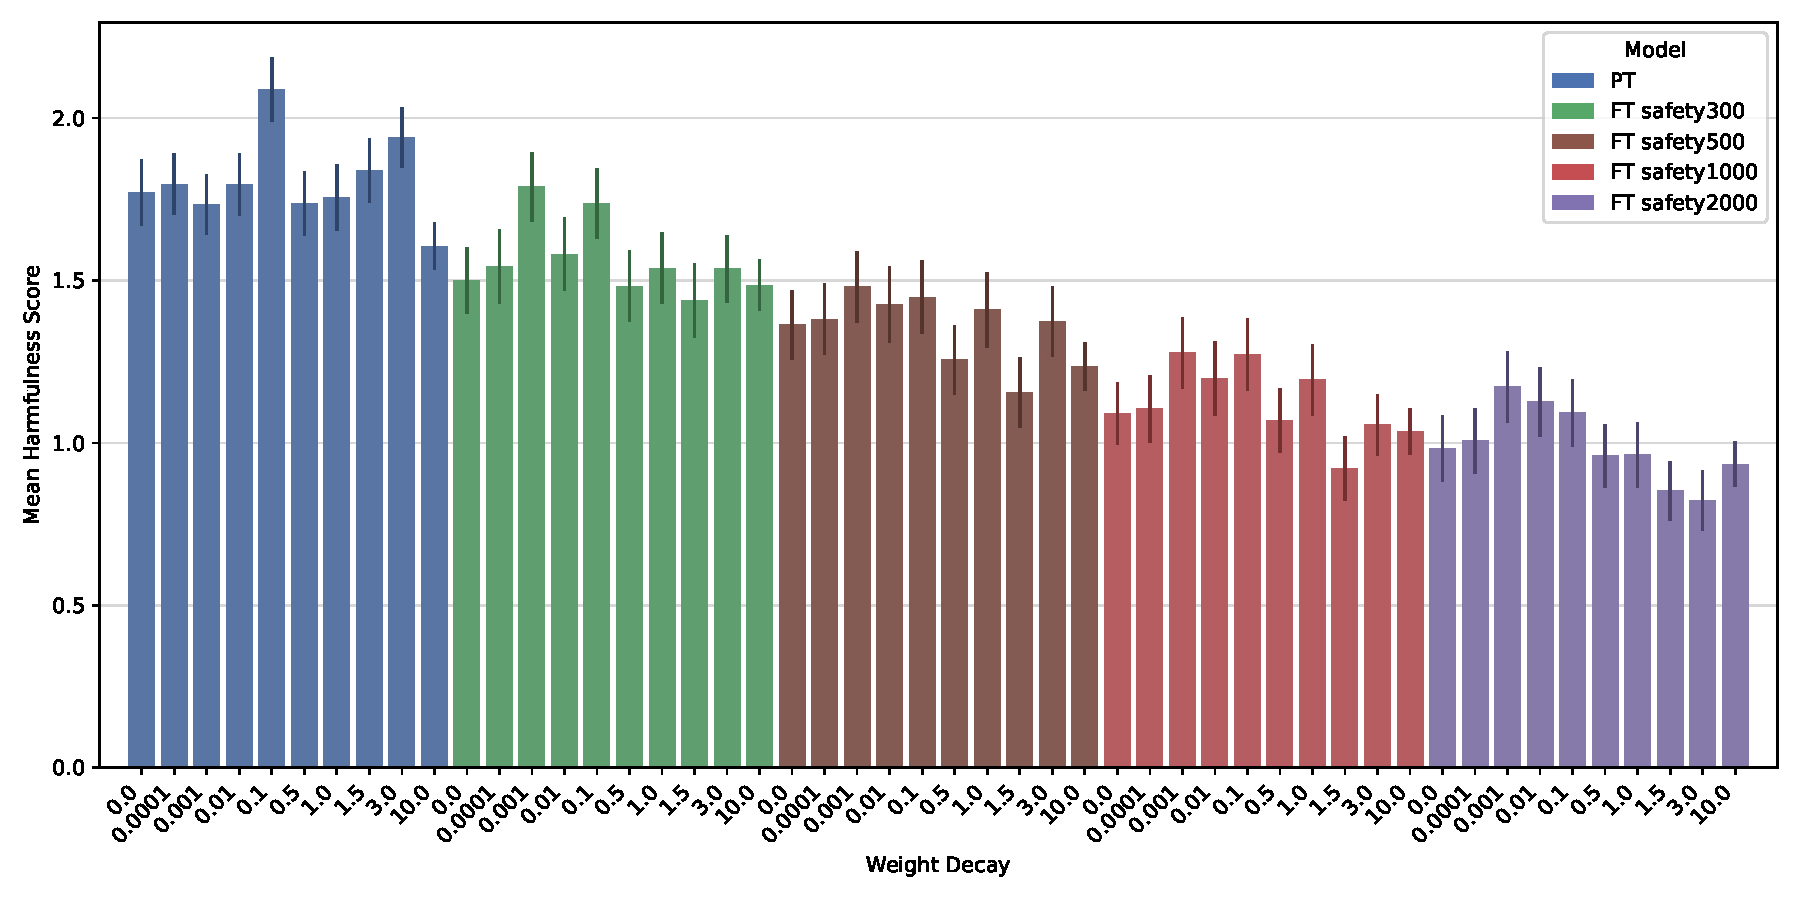
\includegraphics[width=0.55\linewidth]{figs/a11_ft_safety/harmfulness_score_average_llama-1B-20BT.pdf}
    \caption{{\bf Fine-tuning performance for safety alignment.} \llamaoneB{} model.} 
    \label{fig:app-ft-safety-llama1B}
\end{figure}


\begin{figure}[t] 
    \centering
        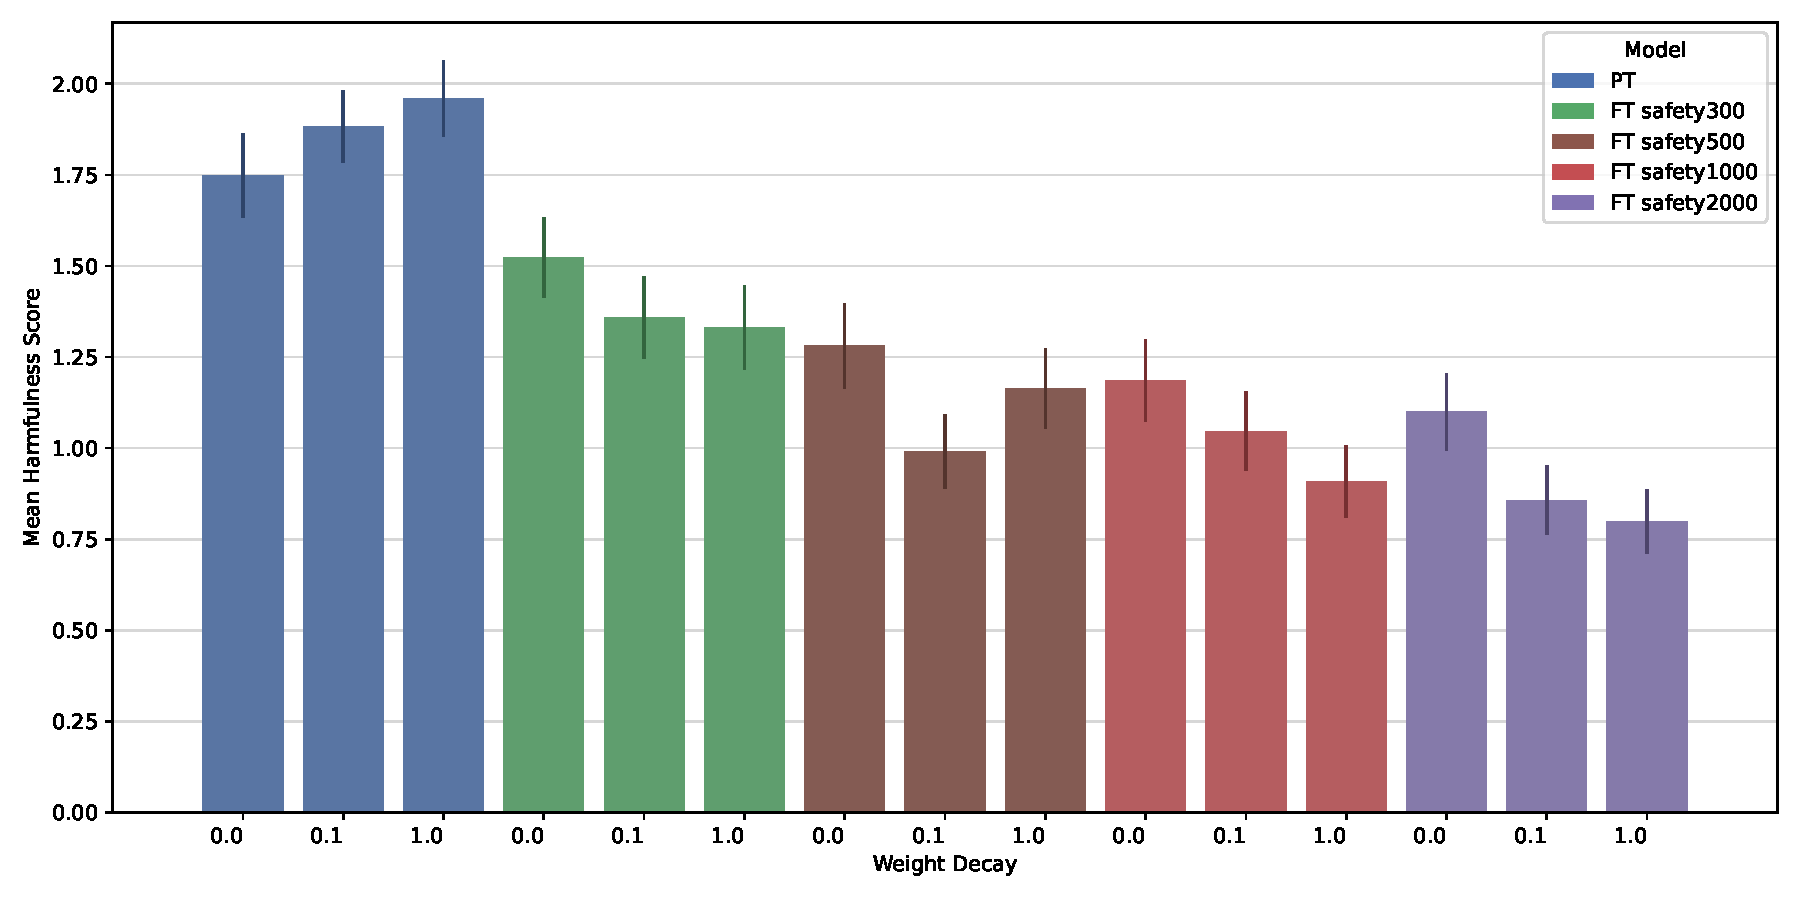
\includegraphics[width=0.55\linewidth]{figs/a11_ft_safety/harmfulness_score_average_llama-4B-80BT.pdf}
    \caption{{\bf Fine-tuning performance for safety alignment.} \llamafourB{} model.} 
    \label{fig:app-ft-safety-llama4B}
\end{figure}

\begin{figure}[t] 
    \centering
        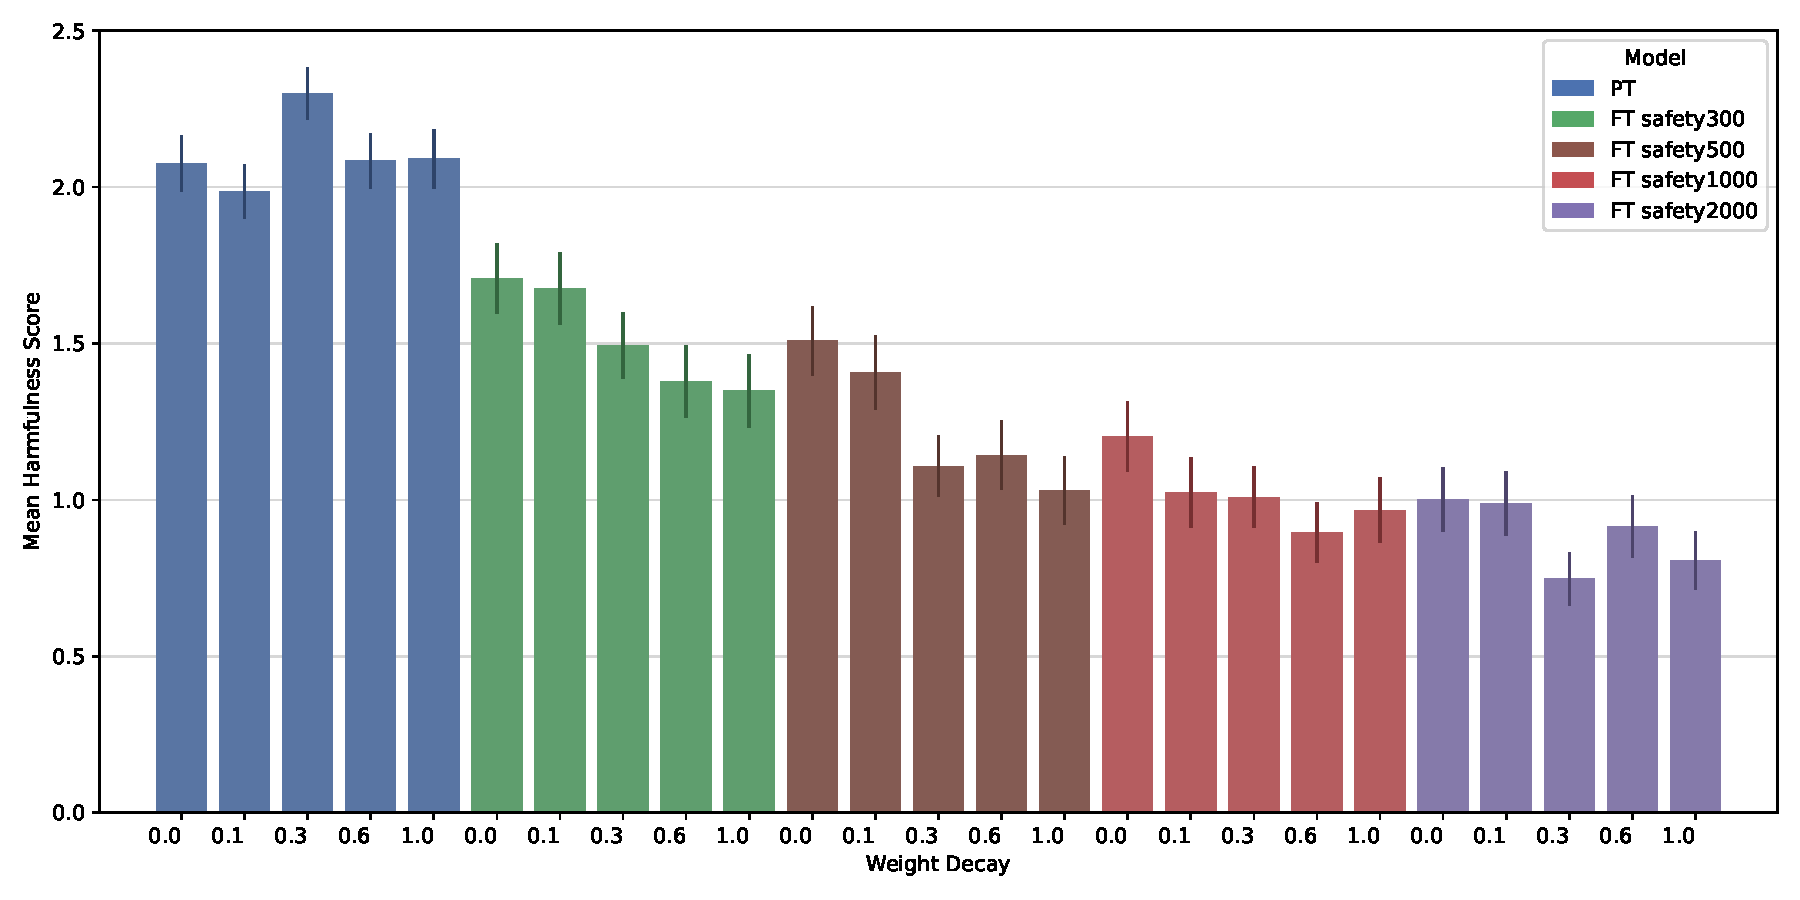
\includegraphics[width=0.55\linewidth]{figs/a11_ft_safety/harmfulness_score_average_olmo-1B-30BT.pdf}
    \caption{{\bf Fine-tuning performance for safety alignment.} \olmoonex{} model.} 
    \label{fig:app-ft-safety-olmo1x}
\end{figure}


\begin{figure}[t] 
    \centering
        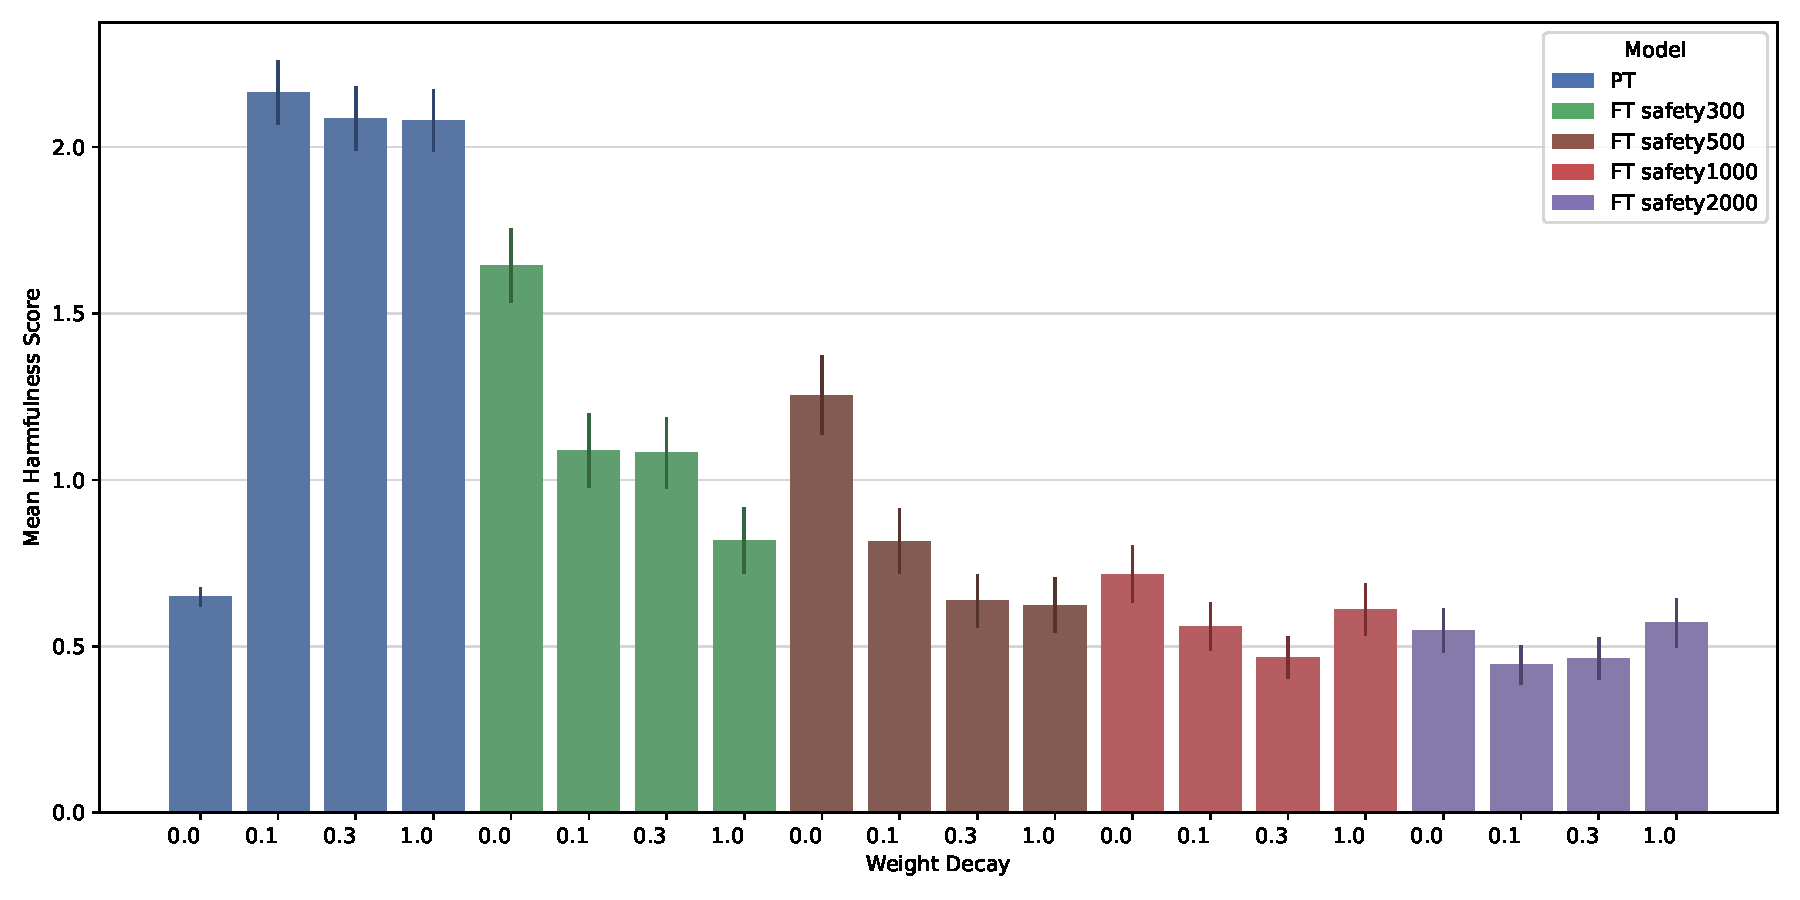
\includegraphics[width=0.55\linewidth]{figs/a11_ft_safety/harmfulness_score_average_olmo-1B-210BT.pdf}
    \caption{{\bf Fine-tuning performance for safety alignment.} \olmosevenx{} model.} 
    \label{fig:app-ft-safety-olmo7x}
\end{figure}

